% The document class supplies options to control rendering of some standard
% features in the result.  The goal is for uniform style, so some attention 
% to detail is *vital* with all fields.  Each field (i.e., text inside the
% curly braces below, so the MEng text inside {MEng} for instance) should 
% take into account the following:
%
% - author name       should be formatted as "FirstName LastName"
%   (not "Initial LastName" for example),
% - supervisor name   should be formatted as "Title FirstName LastName"
%   (where Title is "Dr." or "Prof." for example),
% - degree programme  should be "BSc", "MEng", "MSci", "MSc" or "PhD",
% - dissertation title should be correctly capitalised (plus you can have
%   an optional sub-title if appropriate, or leave this field blank),
% - dissertation type should be formatted as one of the following:
%   * for the MEng degree programme either "enterprise" or "research" to
%     reflect the stream,
%   * for the MSc  degree programme "$X/Y/Z$" for a project deemed to be
%     X%, Y% and Z% of type I, II and III.
% - year              should be formatted as a 4-digit year of submission
%   (so 2014 rather than the accademic year, say 2013/14 say).

\documentclass[ % the name of the author
                author={Aaron Wray},
                % the name of the supervisor
                supervisor={Prof. Dave Cliff},
                % the degree programme
                degree={MEng},
                % the dissertation    title (which cannot be blank)
                title={DeepTrader: A Deep Learning Approach to Training an Automated Adaptive 
                    Trader in a Limit-Order-Book Financial Market},
                % the dissertation subtitle (which can    be blank)
                 subtitle={},
                % the dissertation     type
                type={Research},
                % the year of submission
                year={2020} ]{dissertation}
\usepackage[numbers,sort]{natbib}
\usepackage{mathtools}
\usepackage{subfloat}
\usepackage{subfig}
\usepackage{xcolor}
\usepackage{color, colortbl}
\usepackage{enumitem}
\usepackage{caption}
\usepackage{pdfpages}
\begin{document}

% =============================================================================

% This section simply introduces the structural guidelines.  It can clearly
% be deleted (or commented out) if you use the file as a template for your
% own dissertation: everything following it is in the correct order to use 
% as is.

% \section*{Prelude}
% \thispagestyle{empty}

% A typical dissertation will be structured according to (somewhat) standard 
% sections, described in what follows.  However, it is hard and perhaps even 
% counter-productive to generalise: the goal is {\em not} to be prescriptive, 
% but simply to act as a guideline.  In particular, each page count given is
% important but {\em not} absolute: their aim is simply to highlight that a 
% clear, concise description is better than a rambling alternative that makes
% it hard to separate important content and facts from trivia.

% You can use this document as a \LaTeX-based~\cite{latexbook1,latexbook2} 
% template for your own dissertation by simply deleting extraneous sections
% and content; keep in mind that the associated {\tt Makefile} could be of
% use, in particular because it automatically executes \mbox{\BibTeX} to 
% deal with the associated bibliography. Alternatively, you might want to upload the entire zip folder onto Overleaf (online collaborative \LaTeX platform)



% =============================================================================

% This macro creates the standard UoB title page by using information drawn
% from the document class (meaning it is vital you select the correct degree 
% title and so on).

\maketitle

% After the title page (which is a special case in that it is not numbered)
% comes the front matter or preliminaries; this macro signals the start of
% such content, meaning the pages are numbered with Roman numerals.

\frontmatter

% This macro creates the standard UoB declaration; on the printed hard-copy,
% this must be physically signed by the author in the space indicated.

\makedecl

% LaTeX automatically generates a table of contents, plus associated lists 
% of figures, tables and algorithms.  The former is a compulsory part of the
% dissertation, but if you do not require the latter they can be suppressed
% by simply commenting out the associated macro.

\tableofcontents


% The following sections are part of the front matter, but are not generated
% automatically by LaTeX; the use of \chapter* means they are not numbered.

% -----------------------------------------------------------------------------

\chapter*{Executive Summary}

% {\bf A compulsory section, of at most $1$ page} 
% \vspace{1cm} 

\noindent
% This section should pr\'{e}cis the project context, aims and objectives,
% and main contributions (e.g., deliverables) and achievements; the same 
% section may be called an abstract elsewhere.  The goal is to ensure the 
% reader is clear about what the topic is, what you have done within this 
% topic, {\em and} what your view of the outcome is.

% The former aspects should be guided by your specification: essentially 
% this section is a (very) short version of what is typically the first 
% chapter.  Note that for research-type projects, this {\bf must} include 
% a clear research hypothesis.  This will obviously differ significantly
% for each project, but an example might be as follows:

% \begin{quote}
% My research hypothesis is that a suitable genetic algorithm will yield
% more accurate results (when applied to the standard ACME data set) than 
% the algorithm proposed by Jones and Smith, while also executing in less
% time.
% \end{quote}

\noindent
% The latter aspects should (ideally) be presented as a concise, factual 
% bullet point list.  Again the points will differ for each project, but 
% an might be as follows:

Deep learning neural networks (DLNNs) have proven to be remarkably successful in a number of domains that have previously been challenging for traditional machine learning methods. For example, image classification, speech recognition and natural language processing are areas in which DLNNs have shown superior results compared to other machine learning techniques and in finance, two of the biggest use cases for DLNNs are fraud detection and automated trading.

Over the past 20 years, a number of researchers in industrial and academic research labs around the world have proposed adaptive algorithms for trading, buying and selling in financial exchanges. Trading algorithms implement specific strategies and almost all of the well-known trading algorithms in the literature use either traditional machine-learning or adaptive-control mechanisms. These generally rely on only a small number of observable factors typically focusing almost exclusively on the history of prices quoted in the market. In contrast to traditional machine learning, adaptive algorithms typically use techniques from statistical machine learning to alter their responses to future market events on the basis of their past experience in the market. 

In regards to the nature of the market mechanism, most of the world’s major financial markets are continuous double auction (CDA) systems with a limit order book (LOB). The LOB is a tabular display of the prices and aggregated quantities of all competitive orders (bids or offers) currently posted by traders active in the market.

This project explores the use of DLNNs to train automated adaptive traders which trade on a CDA system that uses a LOB. This is a novel approach because the trading strategy will utilise a lot more data that is available on a LOB than just price information. Specifically, the hypothesis of this research is: 

\begin{quote}
Does the use of DLNNs - specifically recurrent neural networks (RNNs) - and the additional parameters given by a LOB such as the quantities supplied or demanded at each price, and extended time series information on past bids and offers, let us train and create a trading agent that is comparably better than existing trading agents in the public literature?
\end{quote}

This project explores this hypothesis with the intention of answering it under the given time constraints of a master's degree and the limited resources and support received due to the Coronavirus pandemic. The following was completed in compiling this dissertation:
\begin{quote}
\noindent
\begin{itemize}
\item A total of $150$ hours was spent collecting material on and learning about different types of DLNNs, their applications and existing trading agents within the public literature. 
\item An RNN trading agent has been developed and trained using data created from market experiments.
\item An additional $2000$ lines of source code has been written for gathering and cleaning data to be used to train the RNN.
\item Approximately 50,000 market experiments have been conducted in the cloud to obtain data for training.
\item The performance of the RNN trading agent has been compared with traditional trading strategies, commonly referred to by the acronyms AA, GDX, GVWY,SHVR, SNPR, ZIC and ZIP.
\item My results show that the RNN trading agent outperforms or equals the performance of all the following trading strategies: GDX, GVWY, SHVR, SNPR, ZIC and ZIP. My results for AA are ambiguous: in one set of experiments, AA outperforms my trader; in another set, my trader out performs AA. Investigation of this is one direction of future research.


\end{itemize}
\end{quote}

% -----------------------------------------------------------------------------

% \chapter*{Summary of Changes}

% {\bf A conditional section, of at most $1$ page} 
% \vspace{1cm} 

% Iff. the dissertation represents a resubmission (e.g., as the result of
% a resit), this section is compulsory: the content should summarise all
% non-trivial changes made to the initial submission.  Otherwise you can
% omit it, since a summary of this type is clearly nonsensical.

% When included, the section will ideally be used to highlight additional
% work completed, and address criticism raised in any associated feedback.
% Clearly it is difficult to give generic advice about how to do so, but
% an example might be as follows:

% \begin{quote}
% \noindent
% \begin{itemize}
% \item Feedback from the initial submission criticised the design and 
%       implementation of my genetic algorithm, stating ``there seems 
%       to have been no attention to computational complexity during the
%       design, and obvious methods of optimisation are missing within
%       the resulting implementation''.  Chapter $3$ now includes a
%       comprehensive analysis of the algorithm, in terms of both time
%       and space.  While I have not altered the algorithm itself, I
%       have included a cache mechanism (also detailed in Chapter $3$)
%       that provides a significant improvement in average run-time.
% \item I added a feature in my implementation to allow automatic rather
%       than manual selection of various parameters; the experimental
%       results in Chapter $4$ have been updated to reflect this.
% \item Questions after the presentation highlighted a range of related
%       work that I had not considered: I have make a number of updates 
%       to Chapter $2$, resolving this issue.
% \end{itemize}
% \end{quote}

% -----------------------------------------------------------------------------

\chapter*{Supporting Technologies}

This section contains third-party resources and technologies that are used in this project:

\begin{quote}
\noindent
\begin{itemize}
\item The code base of the entire project is written in Python version 2.7 and 3.6.3.
\item To install packages in Python, the Python Package Installer PIP version 20.0.2 was used.
\item The following Python libraries: TensorFlow(2.1.0), Keras(2.3.0), MatPlotLib(3.1.2), Numpy(1.18.2), Seaborn(0.10.0), Boto3(1.13.3) and Progress(1.5).
\item The project uses Cliff’s Bristol Stock Exchange (BSE) to run market simulations and as a test bed to compare trading algorithms.

\end{itemize}
\end{quote}

% -----------------------------------------------------------------------------

\chapter*{Acronyms and Notation}

Notation and Acronyms used throughout this document are as follows:
\subsection*{Acronyms}
\begin{quote}
\noindent
\begin{tabular}{lcl}
% \multirow{3}{*}{Title} \\
AA  &:     & Adaptive Aggressive     \\
AI  &:     & Artificial Intelligence \\
BSE  &:     &  Bristol Stock Exchange \\
CDA  &:     &  Continous Double Auction\\
CNN &:     &  Convulutional Neural Network\\
CSV  &:     &  Comma Separated Values\\
GD  &:     &  Gjerstadt \& Dickhaut\\
GDX &:     &  Gjerstadt \& Dickhaut eXtended\\
DLNN &:     & Deep Learning Neural Network \\
FCNN &:     & Fully Connected Neural Network\\ 
LOB &:     & Limit-Order-Book\\
LSTM &:     & Long Short-Term Memory\\
MBC &:     & Market Based Control\\
MBRA&:     & Market Based Resource Allocation\\
MGD &:     & Modified Gjerstadt \& Dickhaut \\
RNN &:     & Recurrent Neural Network \\
ZI &:     & Zero Intelligence\\
ZIC &:     & Zero Intelligence Constrained\\
ZIP &:     &  Zero Intelligence Plus\\
ZIU &:     &  Zero Intelligence Unconstrained\\

\end{tabular}
\end{quote}
\subsection*{Notation}
\begin{quote}
\noindent
\begin{tabular}{lcl}
$Relu(x)$  &:     & Rectified Linear Unit of $x$\\
$\eta$ &:     &  learning rate\\
\end{tabular}
\end{quote}



% -----------------------------------------------------------------------------

\chapter*{Acknowledgements}
\begin{center}
Firstly, I would like to thank my supervisor who provided me with guidance to help me reach this milestone. Secondly, I would like to thank my girlfriend Frankie for her love and support. Finally, I would also like to acknowledge my brother and parents who provided me with the love, advice and encouragement to help me achieve all of my academic accomplishments.
\end{center}
\mainmatter

% -----------------------------------------------------------------------------

\chapter{Contextual Background}
\label{chap:context}

\section{Introduction}

Auctions are a commonplace mechanism used in trading systems particularly in the financial markets. They are used for the allocation of resources, and for price discovery. The continuous double auction (CDA) is the most commonly used mechanism in financial markets, which also very often make use of a Limit Order Book (LOB) -  a public record of currently active bids and offers. LOBs are implemented globally in many financial exchanges for trading commodities, derivatives, securities and other financial instruments.  

Sales traders play a significant role within financial exchanges. The main function of the sales trader is to buy and sell financial instruments on behalf its clients to obtain the best prices for them whilst receiving a commission on each trade they execute. A key skill to being a successful sales trader is to be adaptive - having the ability to observe the conditions within a market and alter their behaviour accordingly to maximise profit.

In recent times, there has been a great rise in the use of Deep Learning Neural Networks (DLNNs) to solve a variety of problems. DLNNs are a machine learning method inspired by the information processing that occurs within the brain. They have been shown to be effective in numerous applications such as, object detection \cite{object}, speech recognition \cite{speech} and fraud detection \cite{fraud}. Another notable use of neural networks is for time-series analysis where data is analysed at discrete points in time to establish a trend and predict future behaviour \cite{time_series}. 

This project's aim is to apply the use of a DLNN in a unique way to the problem of creating an automated sales trader by using all of the parameters provided by the LOB, to build a trading strategy that is competitive and possibly superior to existing strategies previously published within the public domain. 

Note that some of the extended LOB information that this research uses, is not available to the DLNN at the outset in the real world. The data is not usually collected by the trader in the course of trading and therefore will need to be acquired over a period of time once the strategy is implemented. Nevertheless, the purpose of this research is to ascertain whether a trading advantage over other automated traders could be obtained by collecting and eventually using this data in a DLNN.

\section{Motivation}

\subsection{Economics}

Trade is one of the major building blocks of the world economy. It facilitates global economic growth, the reduction of poverty and increases productivity across the world. It also allows for a greater amount of competition for goods, which leads to lower prices. However, the world economy is a complex system. It consists of an immeasurable number of trades across multiple markets happening concurrently every second. Hence a sophisticated yet dynamic system is required to manage and regulate how these trades are performed across the markets. One of the most effective and commonplace methods of managing these interactions is through the use of financial exchanges.

As financial exchanges act as a marketplace for trading as well as regulating how the trades are executed, they play a vital role in the economy. However for obvious reasons, they are not 100\% efficient. Trades that occur on an exchange are a result of human decisions as well as automated trading agents, which all operate within their own self interest. This can lead to inconsistencies, such as inefficient pricing and resource misallocation. 

Consequently, there are opportunities for arbitrage within the existing system which if exploited successfully can result in financial gain. Moreover, if price discovery can be optimised within these constantly evolving marketplaces this will lead to a more efficient economy and a better society which everyone can prosper and benefit from.



\subsection{Computer Science}

The allocation of resources is not a problem limited to the field of economics. The terms Market Based Resource Allocation (MBRA) or Market Based Control (MBC) describe a set of problems that require fast, robust and distributed control over a resource in a dynamic environment. In the field of Computer Science for example, this is a recurring problem that takes many forms such as sharing out bandwidth in a network or allocating resources to multiple processes in an operating system competing for limited hardware resources. 

A Computer Scientist studies the theory and practical applications of computation, and common problems involving MBRA have been researched extensively. Their job does not stop at finding a solution to a problem, but also about pursuing the one that is most optimal. Artificial Intelligence (AI) is one way of doing just that, a field now widely used to address the problem that is generally considered to have been established at a Dartmouth Summer Research Project in 1956 \cite{Moor_2006}. 

The term machine learning a subset of AI is used to describe methods for computer algorithms to learn from data, and then perform a set of tasks, not necessarily repetitive, without being explicitly programmed to. Machine learning therefore provides a platform to improve existing solutions and solve problems that were thought to be too complex or unpredictable in the past. However, one of the major downsides to the use of AI was thought to be the amount of data required to train AI algorithms as well as the resources required to process it in order to produce desired results. Fortunately, the necessary amount of data and computational power required to train DLNNs is now readily available and, as a consequence, the last few decades has seen a re-emergence in AI, specifically the deep learning a subset of AI. With these developments, DLNNs now present a new and increasingly viable approach to building a strategy for the sales trader problem.

% Economics para talking about  Adam smith paragraph - invisible hand
\section{Previous Work}

\subsection{The Beginning: Experimental Economics}\label{sec:smith}

In 1962, Vernon Smith published an article in the Journal of Political Economy on the experimental study of competitive market behaviour \cite{econ}. The article outlined a number of market simulations based on a CDA mechanism explained further in Section \ref{sec:lob}, where an arbitrary instrument was traded. The supply and demand curves used in theses experiments were realistic, similar to those encountered by real life commodity traders, but were predetermined by Smith. He  achieved this by setting the limit prices for each trader - the price that a buyer cannot buy above and for a seller, the price that a seller cannot sell below. 

The experiments consisted of a small number of human traders, which were divided at random into two subgroups of buyers and sellers. The role of each trader was similar to that of a sales trader i.e. to maximise profit, which in this case is the difference between the price they traded at and their limit price. Each experiment was carried out over a succession of trading ``days'', which lasted between 5 and 10 minutes, depending on the number of traders. 

During each trading day, buyers and sellers would shout out their bids and offers within their given limit prices, much like posting prices to a LOB, except in Smith's early experiments the bids and offers were not recorded. A respective buyer or seller could choose to accept the shouted out bid or offer, or alternatively, a trader could shout out a better price. If a bid/offer was accepted by a trader the trade price was recorded by both parties and both traders would then leave the market, as a trader could only buy or sell a single unit of the instrument being traded. 

The experiments run by Smith demonstrated a rapid convergence of a market to its theoretical equilibrium price (the price where the quantity of goods supplied is equal to the quantity of goods demanded) in a CDA, even with a small number of traders. This was measured by using Smith's $\alpha$. Smith's $\alpha$ is a measure of how well traders in the market collectively discover the equilibrium price. In 2002, Smith received the Nobel Prize for establishing the field of experimental economics and variations of his experiments have been used to test and compare algorithms throughout research on automated trading agents \cite{agent_human, cliff, gode, Rust, AA2}. Likewise, a version of his experiments will be conducted and analysed in this project to support the validity of this research.

\subsection{The Rise of the Automated Trading Agent}\label{sec:rise}
In 1990, a competition was hosted at the Santa Fe Institute for designing the most profitable automated trading agent on a CDA \cite{Rust}. Thirty contestants competed for cash prize incentives totalling \$10,000. The prize money won for each contestant was in proportion to the profit that their agent received in a series of different market environments. The highest ranked algorithm, designed by Todd Kaplan, was a simple agent that would hide in the background and hold off from posting a bid/ask price whilst letting other traders engage in negotiations. Once the bid/ask price was within an adequate range, the Kaplan's agent would then enter and ``steal the deal''. Aptly, his program was named Sniper. During the end of a market session, Kaplan's Sniper would also take advantage of the time left and attempt to make a deal rather than not make one at all.

In 1993, Gode and Sunder investigated the intelligence of automated traders and their efficacy within markets \cite{gode}. They developed two automated trading agents for their experiments, the Zero-Intelligence Unconstrained (ZIU) and the Zero-Intelligence Constrained (ZIC). The ZIU trader generates completely random quote prices, whereas the ZIC trader quotes random prices within a given limit price.

Gode and Sunder's series of experiments were performed in a similar format to Smith's but with different combinations of both human and ZI traders. Three key metrics that were looked at were allocative efficiency, single agent efficiency and profit dispersion. The allocative efficiency is a measure of the efficiency of the market. It is the total profit earned by all traders divided by the maximum possible utility and is expressed as a percentage whereas the single agent efficiency is the profit earned by an agent divided by its expected profit.

Gode and Sunder claimed that their research showed that the ZIC traders were able to equilibriate the market, and that most of the intelligence is in the market and not in the traders, as the allocative efficiency was close to 100\%, irrespective of the traders within the market. Additionally, on the basis of the single agent efficiency the experiments indicated that the ZIC agents were surprisingly human like, which implied that human traders aren't much better than random.

Continuing on from the work of Gode and Sunder, Cliff identified that there were certain market conditions where ZIC traders would fail to equilibriate \cite{cliff}. This finding led him to create an automated trading agent which could converge to the market equilibrium. Consequently in the same paper, he outlined a new automated trader, called Zero Intelligence Plus (ZIP). ZIP is unique when compared with all of the other aforementioned traders, as it incorporates the idea of adaptiveness.

The ZIP trader utilises a profit margin along with a given limit price to calculate an ask/offer price. The profit margin is determined by a learning rule and is adjusted depending on the conditions of the market. If trades are occurring above the calculated price, the profit in margin is increased/decreased depending on whether the trader is a buyer/seller.

In 1998, Gjerstadt and Dickhaut co-authored a paper that approached the sales trader problem from a new perspective \cite{Gjerstad}. They developed a price formation strategy in a CDA that utilized recent market activity to form a belief function. The frequencies of bids, asks, accepted bid and accepted asks from a history of a set number of the most recent trades were used to estimate the belief or probability that an ask or bid would be accepted at a certain price. 

With this strategy, the function selects an ask/offer price that would maximise a trader's expected gain based on the data. The strategy produced efficient allocations and was found to achieve competitive equilibrium within markets. A name was was not given to this strategy in the paper, but in research following from this, it was coined GD (by taking the first initial from both of the author's last names). 

A few years after this, IBM researchers Das and Tesauro modified GD by interpolating the belief function to smooth the function for prices that did not occur in the selected number of recent trades. They named the new trading agent MGD (modified GD) \cite{agent_human}. The IBM paper was the first to explore the interaction between automated trading agents and human traders in a methodical manner, using CDA markets that were close to ones implemented in financial exchanges across the world. 

The trading agents used in their experiments, were ZI traders, Kaplan's Sniper, ZIP, GD and MGD. Both ZIP and MGD consistently surpassed human traders during the experiment. This was an important finding, as at this time sales trading was a job that was only carried out by humans. However since then, a limited amount of research has been carried out about developing an automated trading agent. The majority of this research utilized old-fashioned machine learning techniques and heuristic methods.


One of the few areas of later research was published in 2002 by Tesauro. He followed up on his work on trading strategies by publishing a paper with Bredin that stipulates further alterations to the GD algorithm \cite{gdx}. In the paper, he introduces a new trading strategy, GD eXtended (GDX), which exploits dynamic programming, to learn functions that express long term reward within a CDA.

Further on from this in 2006, Vytelingum created an adaptive aggressive trading agent, named AA, as a part of his PhD research \cite{AA}. The key element of this trading strategy is aggressiveness. A more aggressive trader places a bid/ask that is more likely to be accepted, where as a less aggressive trader will aim to seek a larger gain. This trading strategy estimates the market equilibrium by using a weighted moving average and calculates the volatility of the market by using Smith's $\alpha$.

% Smith's $\alpha$ is the root mean square deviation of a trade around the theoretical equilibrium price \cite{econ}, however the trading strategy uses the estimate of the equilibrium price instead. 

An aggressiveness function is updated based on the price volatility in the market. A more volatile market will give rise to a greater change in bidding behaviour if there is a small change in aggressiveness, whereas a less volatile market will cause a smaller change to bidding behaviour if there is only small change in aggressiveness. Inspired by the work done by Tesauro and Das, De Luca and Cliff ran a series of experiments on the OpEx market simulator, which suggested that AA dominates all known trading strategies \cite{AA2}. However, some years on from this, Snashall and Cliff performed a brute force exhaustive search of all possible permutations of different trading strategies, consisting of over a 1,000,000 market sessions, in order to show that AA doesn't dominate \cite{snashall}. It did show however, that AA was the best performing algorithm over all experiments.

\section{Deep Learning In Finance}\label{sec:deepfin}

As previous mentioned, deep learning is the field that concentrates on solving complex problems through the use of ``deep'' (many-layered) neural networks which is otherwise known as DLNNs. There are many different types of DLNN, each having their own advantages, disadvantages and particular use cases. Nevertheless, DLNNs can be categorised into three main areas: Fully Connected Neural Networks (FCNNs), Convolutional Neural Network (CNNs) and Recurrent Neural Networks (RNNs). A brief discussion of FCNNs and CNNs will be given below, however the latter of the three, RNNs, will be given detailed treatment in this project mainly due to the advantages of using an RNN when processing temporal data. 

It is commonplace to implement RNNs for time series forecasting and a vast amount of research has been completed in this area particularly in spot markets where traders attempt to predict the price of a resource in the future. Predictions are often made to assist in generating a signal on whether a trader should buy, hold or sell the resource that they are trading. 

Although this project employs a DLNN, there is a clear distinction on how it is being used. Rather than being used to predict a future price, this DLNN will be applied to the sales trader problem directly. Put differently, a neural network will be created that will receive a limit price from customer orders, consider the conditions in the market by extracting information from the LOB and finally, given all of this information will produce a price to transact at. Of course in this model, the DLNN is constrained by the limit price from the customer's order, however if the DLNN is to assist the trader in determining a price, it must work within these limitations. 

To the best of my knowledge, there are only two pieces of work that are closely related enough to discuss here. The first is DeepLOB, which uses CNNs which are traditionally used in image processing. Interestingly in this example, CNNs are used to capture the spatial structure of a LOB \cite{Zhang_2019}. In addition to this after processing the information from the LOB, it uses an RNN to examine and take into account information over long periods of time.

Finally, a paper written by le Calvez and Cliff, the most relevant piece of work to this project demonstrates the use of a FCNN to successfully replicate the behaviour of ZIP in a CDA that uses a LOB \cite{le}. It makes the claim of being the the first ever demonstration to successfully replicate a human-like, or super-human, adaptive trader operating in a realistic emulation of a real-world financial market and is a proof-of-concept to show that over time, a DLNN can learn to be better than all of the above.



\section{Project Approach}\label{sec:projectapproach}

One of the fundamental challenges of this project is using an RNN to learn to implement a new trading strategy. Essentially the main ambition lies in applying an RNN in appropriate conditions to create an optimal solution for the sales trader problem. Throughout the literature, claims have been made by the creators of different automated trading agents, that their trading strategy is the best \cite{AA,Gjerstad,gdx}. However, recent research has demonstrated that the best trading strategy mostly depends on the strategies chosen by the rest of the agents within a market \cite{snashall}. Additionally, a vast amount of data is required for an RNN to learn. This is not always readily available to researchers without investing significant resources in terms of cost and data manipulation processing. 

In order to address the data volume requirements of the RNN for the project, the Bristol Stock Exchange (BSE), a LOB based simulation of a financial market, will be the test bed for this project. BSE provides the environment to collect training data needed to train an RNN, by producing information from the LOB throughout a market session. However, choosing the sets of trading strategies that will generate this data, as well as selecting a set of features from the training data need to be given careful consideration as the choices are crucial to the validity of the results across all conditions.

Two further challenges remain in obtaining fair and optimal assessment of any new trading strategy compared to other trading strategies namely identifying circumstances where the strategy underperforms compared to others or whether the strategy is able to equilibriate the market.

To this end, the high-level objective of this project is to use an RNN to create a automated trading agent which is competitive compared to a range of other automated trading strategies and performs well under a number of different trading conditions for the sales trader problem. Essentially, the approach to achieving this will be:

\begin{quote}
\noindent


\begin{enumerate}
\item Research and survey literature on existing automated trading agents.
\item Build on work completed as part of the Applied Deep Learning Unit at Bristol, to further research into the use of RNNs.
\item Implement a data pipeline for the collection and pre-processing of training data from BSE modelling a range of trading conditions.
\item Create a profit making RNN which performs well under differing trading conditions. This will include defining its architecture and methodology, and how it should be initialised.
\item Compare the performance of the new strategy with existing automated trading agents under the various trading conditions, using \textit{balanced-group} and \textit{one-in-many} experiment designs.
\end{enumerate}
\end{quote}

% \begin{quote}
% \noindent
% The high-level objective of this project is to reduce the performance 
% gap between hardware and software implementations of modular arithmetic.  
% More specifically, the concrete aims are:

% \begin{enumerate}
% \item Research and survey literature on public-key cryptography and
%       identify the state of the art in exponentiation algorithms.
% \item Improve the state of the art algorithm so that it can be used
%       in an effective and flexible way on constrained devices.
% \item Implement a framework for describing exponentiation algorithms
%       and populate it with suitable examples from the literature on 
%       an ARM7 platform.
% \item Use the framework to perform a study of algorithm performance
%       in terms of time and space, and show the proposed improvements
%       are worthwhile.
% \end{enumerate}
% \end{quote}

% {\bf A compulsory chapter,     of roughly $5$ pages
% \vspace{1cm} 

% \noindent
% This chapter should describe the project context, and motivate each of
% the proposed aims and objectives.  Ideally, it is written at a fairly 
% high-level, and easily understood by a reader who is technically 
% competent but not an expert in the topic itself.

% In short, the goal is to answer three questions for the reader.  First, 
% what is the project topic, or problem being investigated?  Second, why 
% is the topic important, or rather why should the reader care about it?  
% For example, why there is a need for this project (e.g., lack of similar 
% software or deficiency in existing software), who will benefit from the 
% project and in what way (e.g., end-users, or software developers) what 
% work does the project build on and why is the selected approach either
% important and/or interesting (e.g., fills a gap in literature, applies
% results from another field to a new problem).  Finally, what are the 
% central challenges involved and why are they significant? 
 
% The chapter should conclude with a concise bullet point list that 
% summarises the aims and objectives.  For example:

% \begin{quote}
% \noindent
% The high-level objective of this project is to reduce the performance 
% gap between hardware and software implementations of modular arithmetic.  
% More specifically, the concrete aims are:

% \begin{enumerate}
% \item Research and survey literature on public-key cryptography and
%       identify the state of the art in exponentiation algorithms.
% \item Improve the state of the art algorithm so that it can be used
%       in an effective and flexible way on constrained devices.
% \item Implement a framework for describing exponentiation algorithms
%       and populate it with suitable examples from the literature on 
%       an ARM7 platform.
% \item Use the framework to perform a study of algorithm performance
%       in terms of time and space, and show the proposed improvements
%       are worthwhile.
% \end{enumerate}
% \end{quote}

% -----------------------------------------------------------------------------

\chapter{Technical Background}
\label{chap:technical}

% {\bf A compulsory chapter,     of roughly $10$ pages} 
% \vspace{1cm} 

% \noindent
% This chapter is intended to describe the technical basis on which execution
% of the project depends.  The goal is to provide a detailed explanation of
% the specific problem at hand, and existing work that is relevant (e.g., an
% existing algorithm that you use, alternative solutions proposed, supporting
% technologies).  

% Per the same advice in the handbook, note there is a subtly difference from
% this and a full-blown literature review (or survey).  The latter might try
% to capture and organise (e.g., categorise somehow) {\em all} related work,
% potentially offering meta-analysis, whereas here the goal is simple to
% ensure the dissertation is self-contained.  Put another way, after reading 
% this chapter a non-expert reader should have obtained enough background to 
% understand what {\em you} have done (by reading subsequent sections), then 
% accurately assess your work.  You might view an additional goal as giving 
% the reader confidence that you are able to absorb, understand and clearly 
% communicate highly technical material.



\section{The Limit Order Book}\label{sec:lob}

An English auction, also known as an open ascending price auction, starts with an auctioneer announcing a starting price. Bidders attempt to outbid each other by bidding at the price given by the auctioneer. The auctioneer continuously increases the bid price, until there is only one person with the highest bid. The person with the highest bid wins the auction.

A Dutch auction, also known as an open descending price auction, is the reverse of an English auction. It starts with the auctioneer announcing a start offer-price or ``ask''. However, in this auction the auctioneer progressively reduces the ask price and the first person to accept it wins the auction.

The CDA is a combination of both the English and Dutch auctions, it allows for buyers to be matched with sellers and vice versa. This type of auction very often involves a LOB. A LOB is an anonymised data structure that is consists of two halves: a bids half for buyers to post their bid prices and an asks (offers) half for sellers to post their ask prices. On the buyers half of the LOB prices are listed in descending order with the highest bid price at the top. On the sellers half of the LOB prices are listed in ascending order with the lowest ask price at the top. 

In this way, the best bid and best ask are always at the top of the book. For every price listed the quantity demanded or supplied is also listed beside that price. The LOB may also display the microprice (see Section \ref{sec:terms} for definition) of the traded instrument. Additionally, financial exchanges will also very often use a tape to keep a record of each transaction. For each trade, the tape contains a timestamp, the parties involved and the price it took place at. 

\begin{figure}[H]
    \centering
    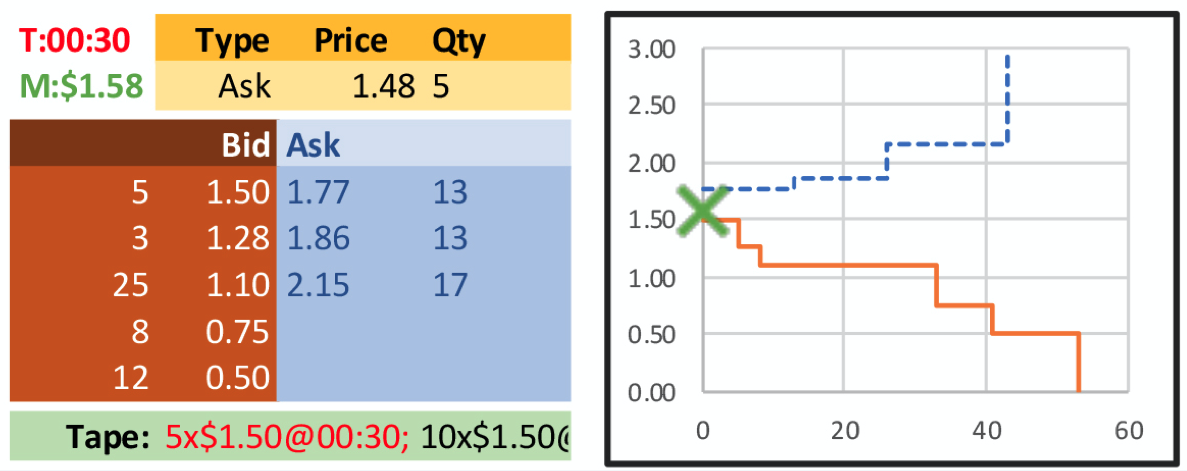
\includegraphics[width=150mm]{bse.png}
   
    \caption{Visualisation of a LOB/tape (left) and the supply/demand curves (right) for a security \cite{bselec}.}
     \label{fig:lobexample}
\end{figure}

The difference between the best ask price and the best bid price is known as the ``spread''. The term ``Crossing the Spread'' is used for when a trade is taking place. A trade occurs if a buyer posts a bid price that is higher than the lowest offer price. This is known as ``lifting the ask'' - the trader wants to buy at the current best ask price. Similarly, if a seller posts an offer price on the LOB lower than the highest bid price, crossing the spread in this direction is known as ``hitting the bid'' - the trader wants to sell at the current best bid price. The information available on a LOB is often referred to as level 2 market data.

Figure \ref{fig:lobexample} displays a LOB for a traded asset 30 seconds into a market session (on the left). There are several bids/asks that have been posted to the LOB. However, a trader has hit the bid by posting an ask of $1.48$ (shown at the top) which is less than the best bid of $1.50$. Therefore, the trader sells the security at best bid price of $1.50$. The transaction is processed by the exchange and information is shown on the tape at the bottom. 

\subsection{Terminology}\label{sec:terms}

The LOB is an extensively researched data structure that contains a lot of information \cite{lob,lob2,AA,cliff, Zhang_2019}. The intention of this section is to provide further clarification, definitions and where appropriate, formulae for key terms associated with both the LOB and for the trading strategies that use it. 

The key terms are listed below:

\begin{itemize}
\item Competitive equilibrium price $p^*$ - first referred to in Section \ref{sec:smith}, is the price at which the supply and demand curves intersect. Stated differently, it is where the quantity demanded of an asset is equal to the quantity supplied.
\item Bid-offer spread - stated in Section \ref{sec:lob} is calculated using the best bid $p_b$ and best ask $p_a$ see in Equation \eqref{eq:spr}. \begin{equation}\label{eq:spr} spread = p_a - p_b\end{equation}
\item Utility $u$ - is the for profit received by a trader. In BSE this is the absolute difference between trade price p and limit price l see in Equation \eqref{eq:util}.\begin{equation}\label{eq:util} u = |p - l|\end{equation}
\item Midprice -  is calculated using the best bid $p_b$ and best ask $p_a$ see in Equation \eqref{eq:mid}. This is the only information that is given by the LOB in level 1 market data. \begin{equation}\label{eq:mid} midprice = \frac{(p_a + p_b )}{2}\end{equation}
\item Microprice - introduced in Section \ref{sec:lob} is an adjustment to the mid-price to take the quantity demanded or supplied  of an asset into account. The microprice is considered to be the more accurate value of an asset than the midprice. It is calculated using the best bid $p_b$, the quantity of the best bid $q_b$, the best ask $p_a$ and the quantity of the best ask $q_b$ see equation \eqref{eq:mic}. \begin{equation}\label{eq:mic} microprice = \frac{(p_b \times q_a) + (p_a \times q_b)}{(q_a + q_b)}\end{equation}

\item Smith's $\alpha$ - described in Section \ref{sec:smith} and \ref{sec:rise} it is used to determine the price volatility in a market. It is the root mean square deviation of the prices $p$ of trades T around the theoretical equilibrium price $p^*$ as shown in Equation \eqref{eq:smith}.\begin{equation}\label{eq:smith} \alpha = \sqrt{\sum_{t \in T}\frac{p_t - p^*}{|T|}} \end{equation}

\item Limit Order Book Imbalance I - determines whether the LOB is bid or ask heavy. The Imbalance is used as indicator for price direction and is calculated using the bid quantity $q_b$ and the ask quantity $q_a$ as in Equation \eqref{eq:imb}. \begin{equation}\label{eq:imb} I = \frac{q_b - q_a}{q_b + q_a}\end{equation}

\item Allocative Efficiency - first mentioned in Section \ref{sec:rise}. Indicates how well the market performed in reaching its competitive equilibrium and is often used as a metric in homogeneous population tests. To calculate the allocative effiency $a$ the total utility earned by all traders $u$ and the theoretical maximum possible utility $u^*$ are needed see Equation \eqref{eq:alleff}. Section \ref{sec:compare} addresses this in further detail.
\begin{equation}\label{eq:alleff} a = \frac{u}{u^*}\end{equation}
\end{itemize}

\section{Bristol Stock Exchange}\label{sec:bse}

The Bristol Stock Exchange (BSE) is a minimal simulation of a limit order book financial exchange. It provides access to level 2 market data and was created by Cliff for teaching and research purposes \cite{cliffbse}. There are several clear distinctions that can be made to distinguish the BSE from a real financial exchange which are outlined below. 

Firstly, there is zero latency. If a trader posts a bid or ask, other traders are able to react to it instantaneously. There is no time between a quote being processed by the exchange and traders being able to respond to it. Secondly, it only permits a trader to submit one type of order, that is a limit order. A limit order is an order to buy/sell at a security at a specific price or better. 
Additionally, BSE only allows a buyer or seller to post a bid/ask with a quantity of one for a traded asset. If a trader is given a new order to execute from a client and posts a quote for it the old quote on the LOB will be deleted, in place of the new one. For each traded asset, the minimum price which can be quoted is 1 and the maximum price that can be quoted is 1000. 

Finally, from the rules given by Smith's experiments, a buyer can only accept offers or post bids less than or equal to its given limit price \cite{econ}. Likewise, a seller can only accept bids or post offers greater than or equal to its given limit price. Therefore, an individual trader is unable to trade at a loss. A trade's profit is the absolute difference between the limit price and the trade price for a security. Despite these aforementioned differences, BSE is an entirely stochastic system that can be used to design experiments and analyse empirical data.

\section{Comparing Strategies}\label{sec:compare}

Comparing the performance of trading strategies is not a straightforward task. As previously mentioned, the performance of a strategy is reliant upon the other traders within the market and in real world financial markets, it is implausible to know what algorithms other traders are using, as this information is confidential. Traders tend not to disclose their strategies in order to remain profitable. Nevertheless, there are methods which can be used to compare trading agents. Tesauro and Das \cite{agent_human} present three separate tests for comparing trading agents two of which will be used in this project:


\begin{itemize}
\item Homogeneous population tests: a test where the market is populated entirely by one trading strategy. Although, this test defines an unrealistic scenario it is used to validate a training strategy and for future reference. Furthermore, it allows us to determine whether a specific trader is able to equilibrate the market. To calculate the allocative effiency of a market, knowledge of the supply and demand curves at all times are required. This would involve calculations after every market event. For this reason, it was thought to be beyond the scope of the project to perform these tests.
\item One-in-many tests: a test where one trader is using a different strategy to the rest. This test is used to explore a trading strategy's vulnerability to invasion and defection. This test will be used to compare DeepTrader with existing strategies in this project.
\item Balanced-group test: a test where buyer and sellers are split evenly with two types of strategy. In addition, every agent of one type of strategy has an identical limit price. This test is considered to be the fairest way to directly compare two strategies. This test will be used to compare DeepTrader with existing strategies in this project.
    
\end{itemize}


\section{Automated Trading Agents}\label{sec:agents}

Section \ref{sec:rise} provided a brief overview of automated trading agents within the literature and only some of the agents used in this project. However, this is not sufficient. A more detailed treatment of trading strategies is required to adequately assess results and make comparisons. The objective of this section therefore, is to deliver a greater insight into all of the automated trading agents used within this project.



\subsection{Giveaway}
The Giveaway trader is an adaption of Gode and Sunder's ZIU agent \cite{gode}. ZIU was designed to pick a completely random quote price and as a consequence, it very often trades at a loss. In the BSE, an individual trader is unable to trade at a loss, so the strategy was modified to ``giveaway'' and only trade at its limit price. The code for the agent is shown in Listing \ref{GVWY}.

\begin{lstlisting}[float=h!,caption=The code for the Giveaway trader,captionpos=b, label=GVWY,language=Python]
# The Order class used to create and handle orders
import Order
# The Trader class used to implement a specific trading strategy
import Trader

class Trader_Giveaway(Trader):
    def getorder(self, time, countdown, lob):
        # checks if the agent has a customer order
        if len(self.orders) < 1:
            # does nothing if there is no customer order
            order = None
        else:
            # sets the quote price as the limit price 
            quoteprice = self.orders[0].price
            order = Order(self.tid, ...)
            self.lastquote=order
        return order
\end{lstlisting}

\subsection{Zero-Intelligence Constrained}
Another trading agent introduced by Gode and Sunder which is also used within this project is ZIC \cite{gode}. ZIC was designed to pick a random quote price that is also within its given limit price and BSE's minimum and maximum price. The code for the agent is shown in Listing \ref{ZIC}.
\begin{lstlisting}[float={h!},caption={The code for the ZIC trader},label={ZIC},language={Python}]
class Trader_ZIC(Trader):
    def getorder(self, time, countdown, lob):
        # checks if the agent has a customer order
        if len(self.orders) < 1:
            # does nothing if there is no customer order
            order = None
        else:
            # assigns the limit price given by the customer order
            limit = self.orders[0].price
            # assigns the order type e.g. bid/ask
            otype = self.orders[0].otype
            
            if otype == 'Bid':
                # generates a random quote price for a bid 
                # The system minimum for a quote price in BSE is 1
                quoteprice = random.randint(1, limit)
            else:
                # generates a random quote price for an ask 
                # The system maximum for a quote price in BSE is 100
                quoteprice = random.randint(limit, 1000)
                
            order = Order(self.tid, ...)
            self.lastquote = order
        return order
\end{lstlisting}

\subsection{Shaver}

The Shaver trading strategy is considered to be an extension of ZIC. The ZIC trader does not utilize any information from the LOB, whereas the Shaver attempts to do just that. The Shaver's approach to the sales trader problem is to always be on the top of the LOB, by having the best bid or ask. To achieve this it ``shaves'' by slightly increasing the current best bid or decreasing the current best ask. In the event that doing this raises it above the limit price for a bid or below the limit price for an ask, the trader acts like Giveaway and just sets the quote price to be the limit price. The code for the agent is shown in Listing \ref{SHVR}.

\begin{lstlisting}[float={h!},caption={The code for the Shaver trader},label={SHVR},language={Python}]
class Trader_Shaver(Trader):
    def getorder(self, time, countdown, lob):
        # checks if the agent has a customer order
        if len(self.orders) < 1:
            # does nothing if there is no customer order
            order = None
        else:
            # assigns the limit price given by the customer order
            limitprice = self.orders[0].price
            # assigns the order type e.g. bid/ask
            otype = self.orders[0].otype
            
            if otype == 'Bid':
                # checks to see if there any bids on the LOB
                if lob['bids']['n'] > 0:
                    # sets the quote price to be the best bid plus one
                    quoteprice = lob['bids']['best'] + 1
                    # checks if the quote price is within the given limit price
                    if quoteprice > limitprice:
                        # assigns the quote price to be the limit price 
                        quoteprice = limitprice
                else:
                    # no bids on the lob so posts the minimum price
                    quoteprice = 1
            else:
                # checks if there are any asks on the LOB
                if lob['asks']['n'] > 0:
                    # sets the quote price to be the best ask minus one
                    quoteprice = lob['asks']['best'] - 1
                    # checks if the quote price is within the given limit price
                    if quoteprice < limitprice:
                        # assigns the quote price to be the limit price 
                        quoteprice = limitprice
                else:
                    # no bids on the lob so posts the maximum price
                    quoteprice = 1000
            order = Order(self.tid, ...)
            self.lastquote = order
        return order
\end{lstlisting}

\subsection{Sniper}

The trading strategy that won the Santa Fe Institute trading agent competition was Kaplan's Sniper \cite{Rust}. Kaplan's Sniper has been modified for BSE and will be referred to as Sniper in this project. Much like the original, Sniper lurks in the background and will attempt to ``steal a deal''. The implementation used for this project is an extension of the Shaver trading agent. Sniper utilizes a countdown parameter which indicates the amount of time left in the market session. The countdown is used to vary amount the Sniper ``shaves'' the best bid or ask by. When a market session is close to ending, the amount the strategy shaves by is reduced in an attempt to make a trade. The code for the agent is shown in Listing \ref{SNPR}.

\begin{lstlisting}[float={h!},caption={The code for the Sniper trader},label={SNPR},language={Python}]
class Trader_Sniper(Trader):

    def getorder(self, time, countdown, lob):
        # parameters used to calculate how much to shave the best bid/ask
        lurk_threshold = 0.2
        shavegrowthrate = 3
        # the amount to shave the best ask/bid by
        shave = 1.0 / (0.01 + countdown / (shavegrowthrate * lurk_threshold))
        # checks if the agent has a customer order
        if len(self.orders) < 1:
            # does nothing if there is no customer order
            order = None
        else:
            # gets the limit price from the customer order
            limitprice = self.orders[0].price
            # gets the type of order e.g. bid/ask
            otype = self.orders[0].otype

            if otype == 'Bid':
                # checks to see if there are any bids on the LOB
                if lob['bids']['n'] > 0:
                    # generates quote price by adding on amount to shave by
                    quoteprice = lob['bids']['best'] + shave
                    # if quote price greater than limit price "giveaway"
                    if quoteprice > limitprice :
                        quoteprice = limitprice
                else:
                    # no bids on the LOB set bid to be min
                    quoteprice = 1
            else:
                # checks to see if there are any asks on the LOB
                if lob['asks']['n'] > 0:
                    # generates quote price by subtracting amount to shave by
                    quoteprice = lob['asks']['best'] - shave
                    # if quote price less than limit price "giveaway"
                    if quoteprice < limitprice:
                        quoteprice = limitprice
                else:
                    # no bids on the LOB set asks to be max
                    quoteprice = 1000
            order = Order(self.tid, ...)
            self.lastquote = order
        return order

\end{lstlisting}
% For problems regarding MBRA, the assumption that all traders will execute the same algorithm is plausible. However, in financial markets homogeneity - where markets are populated entirely by one trading strategy, is implausible. Each trader will operate using their own strategy which ordinarily is kept confidential. 
% -----------------------------------------------------------------------------
% One of the aim's of this project is to not only develop a new trading strategy but to compare it to existing publicly available trading strategies.

\subsection{Zero-Intelligence Plus}

As mentioned previously, Cliff identified that there were conditions that Gode and Sunder's ZI traders failed to equilibriate the market \cite{cliff}. In response to these findings he developed his own trading strategy which could. Namely, ZIP. ZIP directly responds to market events by altering its profit margin $M$ using a learning rule and does this whether or not it has an order. $M$ is used to calculate a percentage multiplier. The multiplier and the limit price $L$ are then used to determine a quote price $P$ seen in Equation \eqref{eq:ZIPe}.

\begin{equation}\label{eq:ZIPe} P = (1\,+M\,)\,\times\,L \end{equation}

For a buyer $M \geq 0$ and for a seller $M \leq 0$, so that the $P$ is always within the given limit price. $M$ is updated throughout a market session using the Widrow-Hoff with momentum learning rule. If trades occur at prices greater than $P$ then $M$ is increased. Alternatively, if trades occur at prices less than $P$, $M$ is decreased. This is done irrespective of a ZIP trader having an order. Thus, ZIP is an adaptive trader as the strategy takes conditions of the market and changes its behaviour.


\subsection{Gerstadt Dickhaut eXtended}

The paper ``Strategic Sequential Bidding in Auctions Using Dynamic Programming'' by Tesauro and Bredin outlines the GDX agent\cite{gdx}. The GDX agent is an extension of the MGD agent that utilizes dynamic programming which computes a belief function $f$ using a history $H$ of $n$ recent trades. The belief function is then used to estimate the probability for each possible bid/ask price $p$ to be accepted at that price. 

The belief function is calculated using: $able(p)$ - the number of accepted bids $\leq p$ in $H$, $ole(p)$ - the number of offers made $\leq p$ in $H$ and $rgbe(p)$ - the number of rejected bids $\geq p$ in $H$ as seen in Equation \eqref{eq:GDX}. The belief function also shows a zero probability for bids lower than the previous lowest trade and for offers higher than the previous highest trade.

\begin{equation}\label{eq:GDX} f(p) = \frac{able(p) + ole(p)}{able(p) + ole(p) + rgbe(p)}\end{equation}
 
The strategy interpolates the belief function over the prices that aren't in $H$ using a cubic spline approach and then uses the belief function on $p$ and the utility $u$ at $p$ to calculate the expected gain $\mu$ as shown in Equation \eqref{eq:GAIN}. The trader sets the quote price to be a value of $p$ that maximises $\mu$.

\begin{equation}\label{eq:GAIN} \mu = f(p) \times u \end{equation}

\subsection{Adaptive Aggressive}

AA is a trading agent developed by Vytelingum in 2006 for his PhD research \cite{AA}. AA was previously was thought to dominate \cite{AA2} until it was shown by Vach and Cliff in 2015 that this may not be true \cite{vach_2015} and altogether disproved by Snashall and Cliff in 2019 \cite{snashall}. Despite this, AA is still considered to be the best performing strategy.

AA calculates an estimate of the competitive equilibrium $\hat{p}^{*}$ of a market session from all trades $T$ using the weighted moving average as in Equation \eqref{eq:AA} \cite{AA}. 

\begin{equation}\label{eq:AA} \hat{p}^{*} = \frac{\sum^T (w_{i} \times p_{i})}{|T|}, \; where \sum^T w_i, \: w_{i-1} = \rho w_i\end{equation}

AA uses an aggressiveness model to calculate the trade price and identifies agents as one of two types. A trader is intra-marginal if it is a buyer and its limit price is higher than the estimated equilibrium price or if it is a seller and its limit price is lower than the competitive equilibrium price. Conversely, a trader is extra-marginal if it is a buyer and its limit price is lower than the estimated equilibrium price or if its a seller and its limit price is higher than the estimated equilibrium price. Intra-marginal traders are more likely to make trades within a market than extra-marginal ones.

The behaviour of the model not only depends on whether the trader is intra-marginal or extra-marginal, it also uses an aggressiveness level $r$. A fully aggressive intra-marginal trader ($r=-1$) makes the bid/ask its limit price in order to trade. An active intra-marginal trader ($r=0$) will attempt to trade at the equilibrium price. A fully passive intra-marginal trader ($r=1$) will quote a price in order to obtain the maximum profit available for a buyer that is the minimum price in the system and for a seller that is the maximum price. 

An extra-marginal trader cannot be aggressive only active ($r=0$) where it will trade at its limit price and passive ($r=-1$) where the agent will try to obtain maximum profit. The aggressiveness level is updated after every bid/ask is posted to the LOB using short term learning rules. Therefore, like GDX and ZIP it is an adaptive strategy.

 \newpage
\section{Deep Learning}\label{sec:deep}

Introduced in Section \ref{sec:deepfin}, Deep Learning is a subset of Machine Learning that utilizes artificial neural networks to extract high level features from input data. The aim of a neural network is to infer a function that performs a specific task. Learning this way is often described as learning ``deep'', hence the name.

Supervised learning involves labelling the data, giving the neural network both input-output pairs so that a neural network can learn the mapping between them. Unsupervised learning requires the data to be unlabelled and only give a network input data, so that the neural network is able to draw inferences and learn the structure of the input data. This project concentrates on the former, as the aim is to use the information provided by running experiments on BSE to learn a mapping from the conditions given by a market and a set limit price to its target - a quote price.

\subsection{The Basics}
In 1958, a form of artificial neural network was invented by Rosenblatt who created the perceptron - a neural network with one hidden layer \cite{rosenblatt1958perceptron}. The perceptron was designed for image/pattern recognition.

Artificial neural networks are made up of three distinct sections: the input layer which is for the input data points, one or more hidden layers which contain a set of neurons and the output layer which produces an output to the problem. A single neuron represents an individual unit of computation.


A neuron is an activation function $f$ and determines whether a neuron is active or not given a set of inputs $x$. Each input is given a specific weight $w$ and the activation function is used to compute an output $y$ on these weighted inputs. This can be seen in Equation \eqref{eq:neuron} where $i$ represents the output from one training example seen by the network. One or typically many neurons are used in combination to produce an output. For simplicity, Section \ref{sec:delta} takes a single layer perceptron with one neuron into consideration. Figure \ref{fig:neuron} shows the example network.



\begin{equation}\label{eq:neuron} y^{(i)}= f(w^T\:x^{(i)}) \end{equation}

\subsection{The Delta Rule}\label{sec:delta}

A network attempts to learn the mapping between input and outputs by updating the weights after seeing each training example. The goal is to obtain the most optimal weights to solve a problem achieved by minimising the error within a network. This is done by performing gradient descent optimisation to adjust the weights within a network. 

\begin{figure}[H]
    \centering
    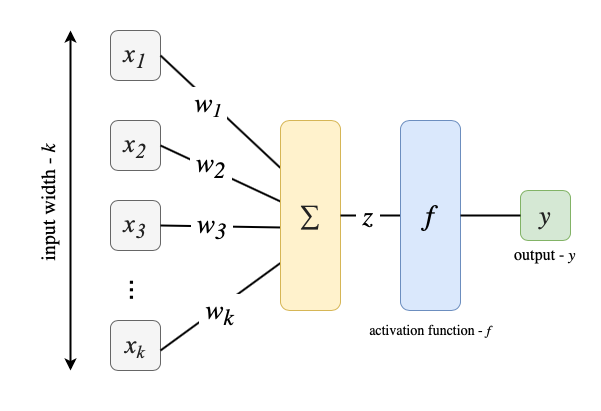
\includegraphics[width=100mm]{neuron.png}
    \caption{Displays a single layer perceptron with one neuron.}
    \label{fig:neuron}
\end{figure}

After the output, also known as the forward activity, has been calculated for a training example, an error function is used to calculate the error $E$ within the network. The error function compares the output of the network $y$, with its true value $v$, to calculate the error. The error function may compute the error in different ways to calculate the network error. In this example, the error function used is the mean squared error and it is given for each training example $i$ as shown in Equation \eqref{eq:mse}.

\begin{equation}\label{eq:mse} E = \frac{1}{2}(v^{(i)} - y^{(i)})^2\end{equation}

To update the weights, gradient descent optimisation is performed. This is done by computing the gradient of the error function with respect to each weight inside of the network. To do this, a few steps are required as described below.

Firstly, the derivative of the weighted inputs $z$ with respect to a weight $w_k$ is the input $x_k$ and the derivative of the weighted inputs with respect to the input $x_k$ is a weight $w_k$ as shown on the left and right of Equation \eqref{eq:weightedinputs} respectively.

\begin{align} \frac{\partial z}{\partial{w_{k}}} &= x_k  &  \frac{\partial z}{\partial x_k } &= w_{k}\label{eq:weightedinputs} \end{align}

Secondly, the activation function of a neuron is typically nonlinear, so that the model can solve problems that are nonlinear. For this example, the sigmoid function is chosen (see the left of Equation \eqref{eq:sigmoid}). Thus, the derivative of the output of the network with respect to the weighted inputs can be determined as shown in the Equation on the right of Equation \eqref{eq:sigmoid}.

\begin{align} y &= \frac{1}{1 + e^{-z}} &  \frac{\partial y}{\partial z} &= y(1-y) \label{eq:sigmoid} \end{align}


The chain rule can then be used with the equations in \eqref{eq:weightedinputs} and \eqref{eq:sigmoid} to find the derivative of the output with respect to each weight in the network see Equation \eqref{eq:chain1}. 

\begin{equation}\label{eq:chain1} \frac{\partial y}{\partial w_k} = \frac{\partial z}{\partial{w_{k}}} \frac{\partial y}{\partial z}  = x_k y(1-y) \end{equation}

Additionally, the derivative of the error function with respect to the output is required.

\begin{equation}\label{eq:error} \frac{\partial E}{\partial y} = (v - y) \end{equation}

One more application of the chain rule with Equations \eqref{eq:chain1} and \eqref{eq:error} gives the derivative of the error function with respect to each weight as in Equation \eqref{eq:chain2}.

\begin{equation}\label{eq:chain2} \frac{\partial E}{\partial w_k} = \frac{\partial y}{\partial{w_{k}}} \frac{\partial E}{\partial y }  = - x_k y(1- y)(v - y)\end{equation}

Finally, applying Equation \eqref{eq:chain2} gives the rule to update the weights inside of the network as shown in Equation \eqref{eq:final}. The learning rate $\eta$ is a configurable hyperparameter which determines how quickly the network learns. 

\begin{equation}\label{eq:final} \Delta w_k = - \eta \, x_k \,\underbrace{y(1- y)(v - y)}_{\text{\normalfont $\sigma$ - error derivative}} \end{equation}

The learning rate has to be selected carefully. Small values can lead to long training times and large values can lead to overfitting. Overfitting is a common problem in Machine Learning and is when a model can only solve a problem for examples that exist within its training set. The model does not generalise well for unseen data. 

Equation \eqref{eq:final} can be reduced to Equation \eqref{eq:widrow-hoff} which is also known as the Delta Rule \cite{widrow1960adaptive}.

\begin{equation}\label{eq:widrow-hoff} \Delta w = - \,\eta\, x \, \sigma \end{equation}

\subsection{The Backpropagation Algorithm}
Section \ref{sec:delta} discusses a network with one hidden layer. However, in order to learn ``deep'' and extract more features from input data, more hidden layers are required. Unfortunately though, for neural networks with more than one hidden layer, the problem of finding the error within in a network with respect to each weight or computing the steepest descent, becomes more complicated. Each hidden unit can have an effect on the output and therefore the effect of each hidden layer on the output has to be combined in some way. 

An efficient way of solving this problem is by using the Backpropagation algorithm which utilizes dynamic programming \cite{backprop}. It computes the error derivatives of one layer and then uses that to compute the error derivatives for the layer below ``backpropagating'' the error throughout a network.

Continuing on from Section \ref{sec:delta}, the sigmoid activation and mean squared error functions are used to achieve this. Equation \eqref{eq:final3} shows the new rule for updating weights where $i$ and $j$ represents a neuron from an individual layer. Additionally, the network sums the partial derivative for batches of training examples to compute the weight update.

\begin{equation}\label{eq:final3} \Delta w_{ij} = - \sum_{batch} \,\eta \,y_i\, y_j\, (1- y_j)\frac{\partial E}{\partial y_j} \end{equation}


\subsection{Long Short-Term Memory Recurrent Networks}

Recurrent Neural Networks RNNs are designed for processing sequential data. RNNs are different from a regular neural network because they share the weights between all previous members of the output. In other words, weights are shared across time which makes RNNs ideal for processing temporal data. However, this leads to an even ``deeper" computational graph, as not only do we have to consider the effect of each parameter on the output, the parameters from a previous time $t$ have to also be considered.

Training an RNN is even more complicated then a regular fully connected neural network. To compute the gradient of the error function with respect to each weight in an RNN, the forward activity of the network at each time $t$ has to be computed. The forward activity is then stored and used to backpropagate the error through all time steps. This algorithm is known as backpropagation through time.

In 1991, Hochreiter identified that RNNs suffer from the fundamental problem of deep learning: vanishing/exploding gradients \cite{vanish}. Gradients propagated over time tend to vanish or explode at an extremely large rate such that the weights no longer have an affect on learning. Thus, causing a failure for a network to learn.

In 1997, Hochreiter and Schmidhuber published a paper on Long Short-Term Memory (LSTM) networks demonstrating a form of gated RNN which overcame the problem of vanishing/exploding gradients \cite{LSTM}. An LSTM captures the long term dependencies between time steps by using forget gates. A forget gate uses the sigmoid function (see the left of Equation \eqref{eq:sigmoid}) to give an LSTM the ability to forget old states when necessary. Furthermore, it allows an LSTM to capture both the short and long term dependencies, but more specifically, the long term dependencies between inputs without the effect of vanishing/exploding gradients.


\section{Summary}

This chapter has provided a detailed technical overview of the sales trader problem and some of the existing strategies that have been used to solve it. Additionally, it outlines research completed on Deep Learning. Its intention has been to provide the reader with the technical understanding required to achieve the goal of this project namely to apply a Deep Learning methodology to the sales trader problem through the use of a LSTM network and to compare the new trading agent with existing strategies.

\cleardoublepage

\chapter{Project Execution}
\label{chap:execution}

\section{Bristol Stock Exchange Modifications}\label{sec:bseexec}

As first introduced in Section \ref{sec:bse}, BSE is the test bed for this project. BSE was used to collect all of the data required to train the LSTM network for DeepTrader and then test its performance against existing trading strategies. BSE is written in Python 2.7 and therefore, for compatibility reasons, the majority of this project is also written in Python 2.7. There are a few notable exceptions namely some data preprocessing work, running BSE in the cloud and preliminary training of the LSTM network. These components can be considered to be independent of developing a trading strategy for BSE and for the reasons of usability and in some cases speed, they are all written in Python 3.6. 

\subsection{Training Data Price Ranges}\label{sec:ranges}

In order to mimic the real world, BSE enables a user to control the supply and demand schedules for a market session. This includes the maximum and minimum price ranges for a customer's order. To expose DeepTrader to a wide range of supply and demand curves rather than avoiding a repetition.

\subsection{Feature Selection}\label{sec:features}
BSE produces data throughout a market session, and monitors the profit per trader. This data is recorded for every trader in a market session and the output is written to a file in CSV format. However, this data is insufficient to train an LSTM network to trade on a market. 

After reviewing the literature and performing research (see sections \ref{sec:smith} and \ref{sec:agents}), 14 additional features were extracted from BSE and output to the CSV file to train the LSTM network for each trade that occurred within a market session. These are as follows:

\begin{enumerate}[leftmargin=*,labelindent=16pt]
    \item The time $t$ the trade took place after the market session began in seconds.
    \item A binary representation of the customer order type that was used to generate the quote, that initiated the trade (1 for bid and 0 for ask).
    \item The limit price of the customer order that was used to generate the quote that initiated the trade.
    \item The bid-ask spread on the LOB at time $t$ defined in Section \ref{sec:terms} if undefined set to 0.
    \item The midprice of the LOB at time $t$ defined in Section \ref{sec:terms} if undefined set to 0.
    \item The microprice of the LOB at time $t$ defined in Section \ref{sec:terms} if undefined set to 0.
    \item The best (highest) bid on the LOB at time $t$ if undefined set to 0.
    \item The best (lowest) ask on the LOB at time $t$ if undefined set to 0.
    \item The difference in time between the previous and current trade, for the first trade this is the trade price.
    \item The LOB imbalance at time $t$ defined in Section \ref{sec:terms}.
    \item The total quantity of all quotes on the LOB a time $t$.
    \item An estimate of the competitive equilibrium price at time $t$ as defined by Vytelingum \cite{AA} see Equation \eqref{eq:AA}.
    \item Smith's $\alpha$ calculated by using an estimate of the competitive equilibrium price at time $t$ defined in Section \ref{sec:terms}.
    \item The price of the trade.
\end{enumerate}

The first 13 items in the list are the multivariate input to the network. Item 14 is the output (target) variable that the network is training toward. 

A single CSV file was generated to store the data for all trades in one market session. A high volume of data was therefore generated for the many market sessions required to train the DLNN. To handle the heavy data and processing requirements, the market sessions were ran in the cloud.


\section{Data Collection}\label{sec:cloud}

Section \ref{sec:agents} details all seven trading agents contained in BSE that were used in this project. To create a large dataset to train the model, many markets session configurations were devised where the proportions and types of traders were varied. 

\newcommand\Myperm[2][^n]{\prescript{#1\mkern-2.5mu}{}P_{#2}}
\newcommand\Mycomb[2][^n]{\prescript{#1\mkern-0.5mu}{}C_{#2}}

Each market session had 80 traders (40 buyers and 40 sellers). Additionally, each market session used four different trading strategies. For each trading strategy, the number of buyers and sellers was always the same but there were five different proportion groups of traders used. These proportions groups were: (20, 10, 5, 5), (10, 10, 10, 10), (15, 10, 10, 5), (15, 15, 5, 5) and (25, 5, 5, 5). Each number within a group denotes the number of buyers and sellers for a specific trading strategy within a market session. As an example the (20, 10, 5, 5) proportion group, indicates that there were 20 buyers and sellers of trading strategy 1; 10 buyers and sellers of trading strategy 2; 5 buyers and sellers of trading strategy 3; and 5 buyers and sellers of trading strategy 4 within this group.
Given that there are 4 trading strategies in each session selected from a total pool of 7 available strategies, gives a total of 35 different combinations ($\prescript{7\mkern-0.5mu}{}C_{4}$) of trading strategies.

Furthermore, there are 35 different permutations for each of the proportion groups listed. This led to a total of 1225 (35 x 35) different market configurations where the proportions and types of traders were varied. Each market configuration was executed 32 times with different random-number sequences for additional variability giving a total of 39,200 different market sessions.

This multiple implementation method of BSE is not ideal from a processing perspective as each individual market session takes approximately 30 seconds to complete, so running all 39,200 on a single computer would take approximately 13.5 days. For this reason, the decision was made to use Amazon's Elastic Compute Cloud (EC2) service to parallelise data collection processes amongst 32 virtual machines (instances). The Python library Boto3 (1.13.3) was used to create, manage and terminate the EC2 instances. The work was split amongst each instance by making every instance run each market configuration once and used a separate custom utility, created for this project, to automate the process.

\section{Data Preprocessing}
The Pickle library was used to convert all CSV files produced from running the market sessions into one large continuous stream of bytes to save time when loading the dataset for training.

 All of the data features used in training the DLNN have been previously outlined in Section \ref{sec:features}. However each feature can have values within differing ranges.  In this implementation, a single input consists of 13 different features and the contribution of one feature depends on its variability relative to other features inside of the input. If for example, one feature has a range of 0 to 1, while another feature has a range of 0 to 1,000, the second feature will have a much larger effect on the output. Additionally, values in a more limited range (e.g. 0 to 1) will result in faster learning.

Therefore, when training a multivariate neural network such as in this implementation, it is common practice to normalise all features in the training dataset such that all values are within the same scale. The normalisation method chosen here was min-max normalisation. Min-max normalisation scales all data in the range $[0,1]$, by using the minimum and maximum values for each feature $X$ in the training data. In this way, it does not alter any distribution within the data. The equation used to normalise each feature is shown in Equation \eqref{eq:normalise}, where $i$ denotes a single training example.
\begin{equation}\label{eq:normalise}X_{norm} = \frac{X_{i}-X_{min}}{X_{max}-X_{min}} \end{equation}
Typically, neural networks have train, validation and test datasets. The train dataset is used to train the model and is the data that a neural network learns from, whilst the validation dataset is used for tuning a model's hyperparameters and the test dataset is used to evaluate a model's final performance. For this project, as the performance of the neural network is determined by how well it trades during a market session, there is no distinct test dataset. Alternatively, the split of the test and validation datasets will be 90\%:10\% respectively from the data collected.

\section{Network Architecture}


The LSTM network created consists of three distinct hidden layers. The first hidden layer is an LSTM layer containing 10 neurons. The final two hidden layers are both fully connected layers containing 5 and 3 neurons respectively. Each hidden layer uses the Rectified Linear Unit (Relu) as an activation function as described by equation \eqref{eq:relu}.
\begin{equation}\label{eq:relu} Relu(x) = max(0,x) \end{equation}

\section{Training}
The train dataset was too large to use all data points at once. The process is limited by the size of memory on the machine used to train the netowork. Therefore, was training was executed in batches. Each batch consisted of $16384$ data points and the Adam optimiser is used to train the network. As previously discussed in in section \ref{sec:delta}, learning rates require careful selection, and Adam uses an adaptive learning rate method that calculates different learning rates based on the weights in the network. The initial learning rate $\eta = 1.5\times10^{-5}$ which is a reasonable compromise between overfitting and long processing times. 

The function that was used to calculate the error (loss) within the network was the mean squared error (MSE) given in Equation \eqref{eq:mse}. An epoch can be considered as the model seeing each data point within the dataset once. The model was trained for 20 epochs and the loss after each training epoch is shown in Figure \ref{fig:loss} below.

\begin{figure}[H]
    \centering
    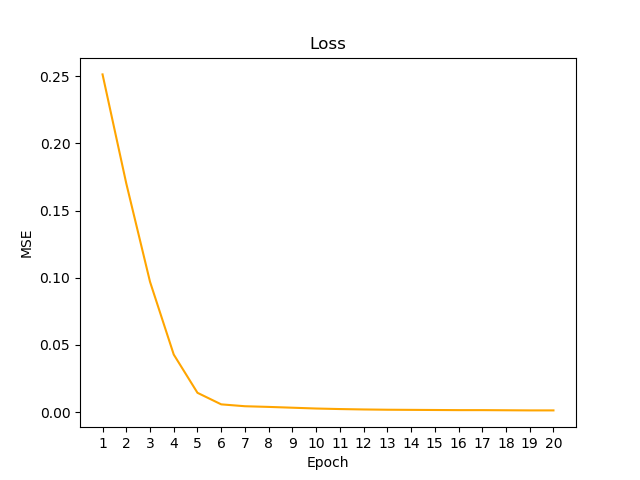
\includegraphics{loss_train.png}
    \caption{MSE loss after each training epoch}
    \label{fig:loss}
\end{figure}

\section{DeepTrader}
DeepTrader uses the information provided by the LOB specified in Section \ref{sec:features} and a customer order's given limit price to calculate a price to trade at. However, it first has to normalise inputs before this information is used, in the same way as the training data. Consequently, the minimum and maximum values for all features within the training data are stored and loaded from a file so that they can be used to normalise the input to the model. Once DeepTrader has determined the price, the output will be in the range [0,1]. Therefore, the output is ``denormalised'' to produce a trade price that is appropriate for BSE. Listing \ref{eq:normalise} shows the algorithm used for denormalistaion.

\begin{lstlisting}[float={h!},caption={The getorder Function of DeepTrader},captionpos={b},label={DTR},language={Python}]
class DeepTrader(Trader):
    def getorder(self, time, countdown, lob):

        if len(self.orders) < 1:
            # no orders: return NULL
            order = None
        else:
            qid = lob['QID']
            tape = lob['tape']
            otype = self.orders[0].otype
            limit = self.orders[0].price

            # creating the input for the network
            x = self.create_input(lob)
      
            normalized_input = (x-self.min_vals[:self.n_features]) / (
                self.max_vals[:self.n_features]-self.min_vals[:self.n_features])
            normalized_input = np.reshape(
                normalized_input, (1, 1,-1))

            # retrieving the networks output
            normalized_output = self.model.predict(normalized_input)[0][0]
            # denormalizing the output
            denormalized_output = ((normalized_output) * (
                self.max_vals[self.n_features] 
                - self.min_vals[self.n_features]))
                + self.min_vals[self.n_features]
            model_price = int(round(denormalized_output, 0))

            if otype == "Ask":
                if model_price < limit:
                    self.count[1] += 1
                    model_price = limit
            else:
                if model_price > limit:
                    self.count[0] += 1
                    model_price = limit

            # print(seld.tid, self.count)

            order = Order(self.tid, ...)
            self.lastquote = order
        return order
\end{lstlisting}

\section{Experiments}\label{sec:results}
Section \ref{sec:compare} outlined three different methods of comparing trading strategies. The most appropriate methods were deemed to be one-in-many tests and balanced-group tests for reasons highlighted in that section. Additionally, the most significant measure used when analysing and comparing the performance of trading agents is the amount of profit received per type of trader. Therefore, this is the key metric collected during the course of the experiments that are described in this section.

\subsection{Balanced Grouped Tests}
The Balanced Group Tests were carried out using DeepTrader and the other traders that exist within BSE. These tests consisted of 100 iid market sessions and each market session contained 20 buyers and 20 sellers of one type of trader. The ranges for limit prices are set in the same way as when the training data was collected (see section \ref{sec:cloud}). Figure \ref{fig:balanced} shows box plots of results for the various balanced group configurations. 

For each box plot, the edge of the box displays the upper and lower quartiles, the line inside of the box shows the median of the dataset and the whiskers extend to show the rest of the distribution. Except, any data point that is a distance of 1.5 multiplied inter-quartile range from the upper or lower quartiles respectively is classified as an outlier. Outliers are represented on the box plots as diamonds.

\begin{figure}[h!]
   
    \centering
    \subfloat[Box plot to display profit per trader from the balanced group tests with DeepTrader and the ZIP trader.]{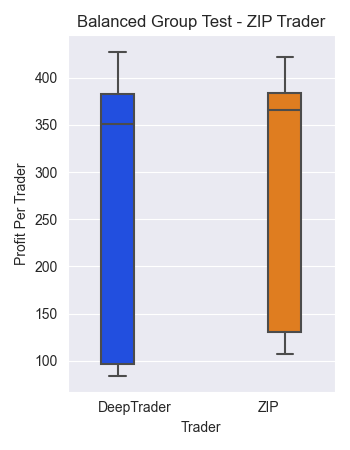
\includegraphics[width=3.1in]{Balanced Group Test - ZIP Trader.png}} \label{fig:bZIP}
    \captionof{figure}{Balanced Group Test Results}
    \label{fig:balanced}
\end{figure}

\begin{figure}[h!]
    \ContinuedFloat
    \subfloat[Box plot to display profit per trader from the balanced group tests with DeepTrader and the AA trader.]{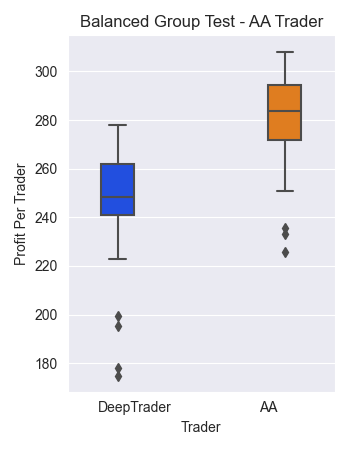
\includegraphics[width=3.1in]{Balanced Group Test - AA Trader.png}}\label{fig:bAA}
    \subfloat[Box plot to display profit per trader from the balanced group tests with DeepTrader and GDX trader.]{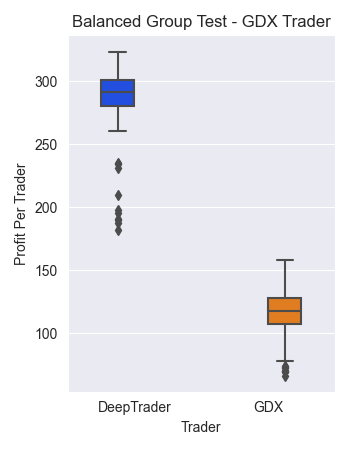
\includegraphics[width=3.1in]{Balanced Group Test - GDX Trader.png}} \label{fig:bgdx}
\end{figure}

\begin{figure}[h!]
    \ContinuedFloat
    \centering
    \subfloat[Box plot to display profit per trader from the balanced group tests with DeepTrader and the Giveaway trader.]{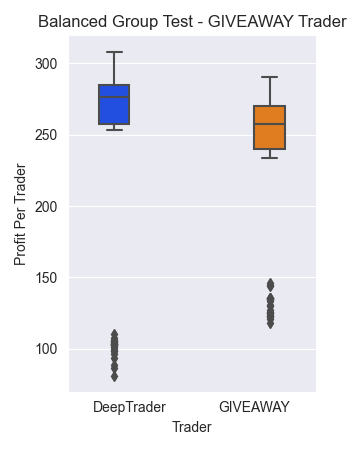
\includegraphics[width=3.1in]{Balanced Group Test - GIVEAWAY Trader.png}}\label{fig:bGVWY}
    \subfloat[Box plot to display profit per trader from the balanced group tests with DeepTrader and the Shaver trader.]{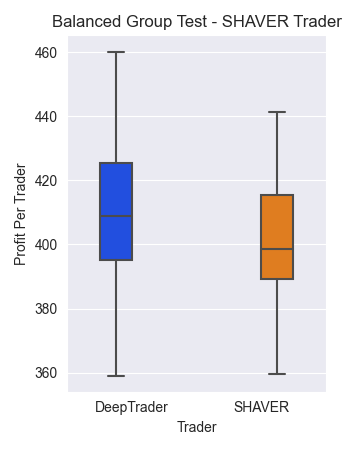
\includegraphics[width=3.1in]{Balanced Group Test - SHAVER Trader.png}}\label{fig:bshave} \\
    \subfloat[Box plot to display profit per trader from the balanced group tests with DeepTrader and the Sniper trader.]{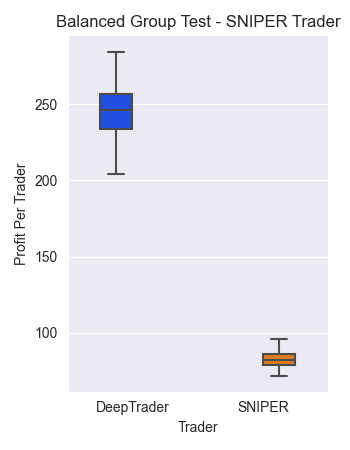
\includegraphics[width=3.1in]{Balanced Group Test - SNIPER Trader.png}} \label{fig:bsniper}
    \subfloat[Box plot to display profit per trader from the balanced group tests with DeepTrader and the ZIC trader.]{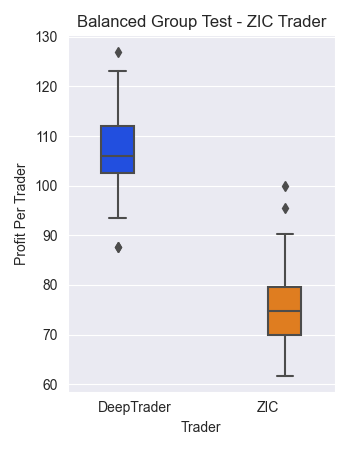
\includegraphics[width=3.1in]{Balanced Group Test - ZIC Trader.png}}\label{fig:bZIC} \\
   
  
    
\end{figure}

\subsection{One In Many Tests}
The One In Many test were also carried out using DeepTrader and the traders that exist within BSE. Again, these tests consisted of 100 iid market sessions. Each market session contained 1 DeepTrader buyer and 1 DeepTrader seller and 39 buyers and 39 sellers of another type of trading strategy. The ranges for limit prices are set in the same way as when the training data was collected (see Section \ref{sec:cloud}). Figure \ref{fig:one} below show box plots of results for the various one-in-many configurations.


\begin{figure}[h!]
  
    \centering
    \subfloat[Box plot to display profit per trader from the one in many tests with DeepTrader and the ZIP trader.]{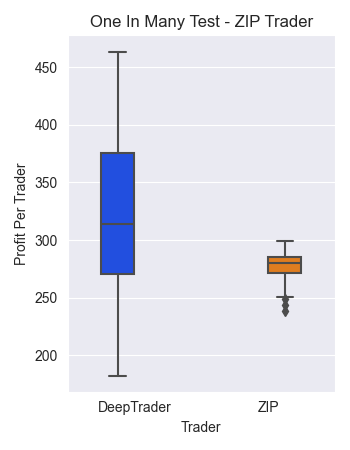
\includegraphics[width=3.1in]{One In Many Test - ZIP Trader.png}} \label{fig:oZIP}
   
    
    \captionof{figure}{One In Many Test Results}
    \label{fig:one}
\end{figure}
\begin{figure}[h!]
    
    \ContinuedFloat
    \centering
    \subfloat[Box plot to display profit per trader from the one in many tests with DeepTrader and the ZIP trader.]{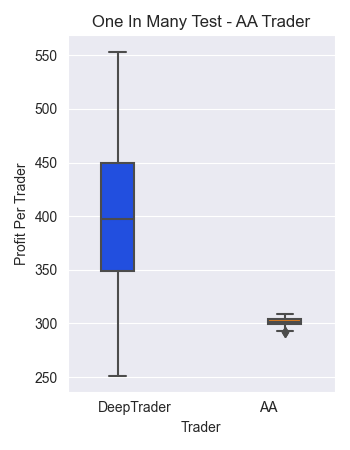
\includegraphics[width=3.1in]{One In Many Test - AA Trader.png}} \label{fig:oAA}
    \subfloat[Box plot to display profit per trader from the one in many tests with DeepTrader and the ZIP trader.]{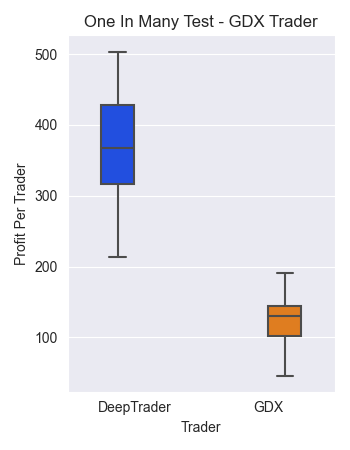
\includegraphics[width=3.1in]{One In Many Test - GDX Trader.png}} \label{fig:oGDX}
\end{figure}
\begin{figure}[h!]
    \ContinuedFloat
    \centering
    \subfloat[Box plot to display profit per trader from the one in many tests with DeepTrader and the Giveaway trader.]{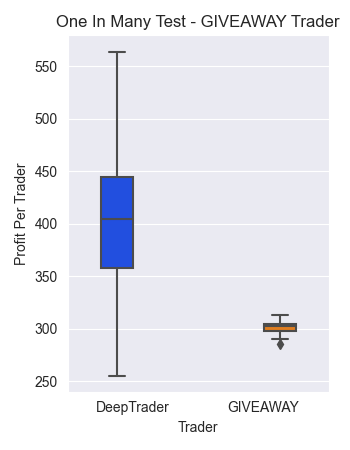
\includegraphics[width=3.1in]{One In Many Test - GIVEAWAY Trader.png}}\label{fig:oGVWY}
    \subfloat[Box plot to display profit per trader from the one in many tests with DeepTrader and the Shaver trader.]{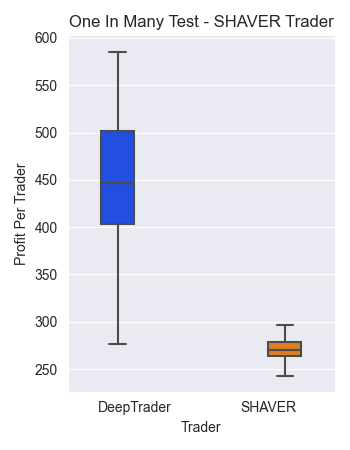
\includegraphics[width=3.1in]{One In Many Test - SHAVER Trader.png}}\label{fig:oshave} \\
    \subfloat[Box plot to display profit per trader from the one in many tests with DeepTrader and the Sniper trader.]{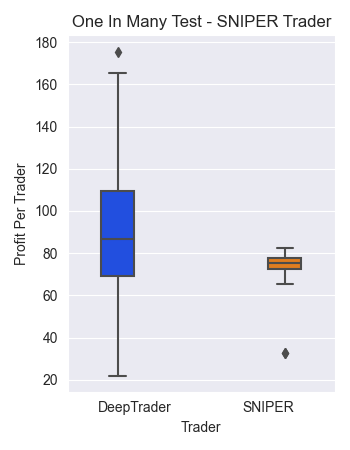
\includegraphics[width=3.1in]{One In Many Test - SNIPER Trader.png}} \label{fig:osniper}
    \subfloat[Box plot to display profit per trader from the one in many tests with DeepTrader and the ZIC trader.]{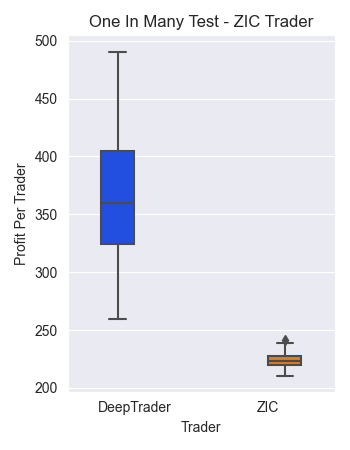
\includegraphics[width=3.1in]{One In Many Test - ZIC Trader.png}}\label{fig:oZIC} \\

    
\end{figure}
\clearpage
\section{Summary}

This chapter establishes the actions completed in the project in order to successfully develop the DeepTrader strategy. In addition, a detail description of the experiments performed to compare DeepTrader with existing strategies was provided. Chapter \ref{chap:evaluation} aims to provide statistical analysis from the experiments described.
% \begin{figure}[H]
%   \centering
%   \begin{tabular}
%     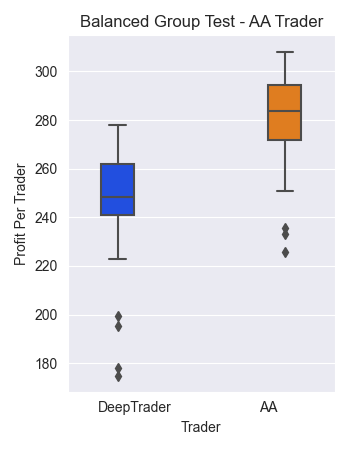
\includegraphics[width=.3\linewidth,height=120pt]{Balanced Group Test - AA Trader.png}
%     \caption{Coffee.}
%   \end{tabular}
%   \begin{tabular}
%     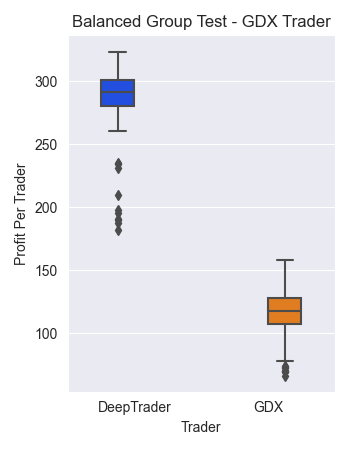
\includegraphics[width=.3\linewidth,height=120pt]{Balanced Group Test - GDX Trader.png}
%     \caption{More coffee.}
%   \end{tabular}
%   \begin{tabular}
%     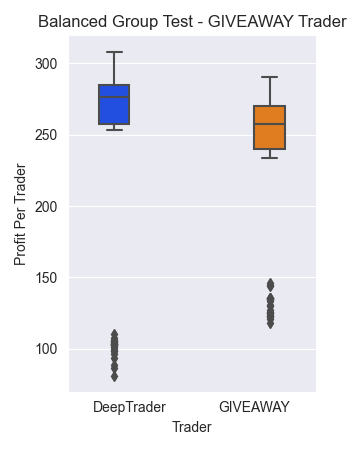
\includegraphics[width=.3\linewidth,height=120pt]{Balanced Group Test - GIVEAWAY Trader.png}
%     \caption{Tasty coffee.}
%   \end{tabular}
%   \begin{tabular}
%     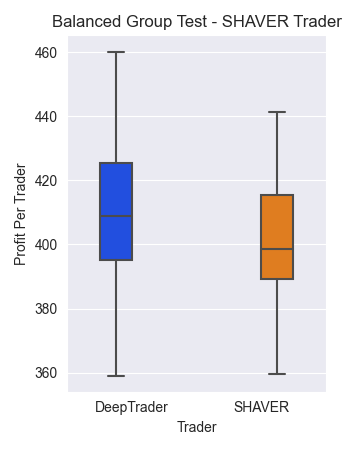
\includegraphics[width=.3\linewidth,height=120pt]{Balanced Group Test - SHAVER Trader.png}
%     \caption{Too much coffee.}
%   \end{tabular}
%   \begin{tabular}
%     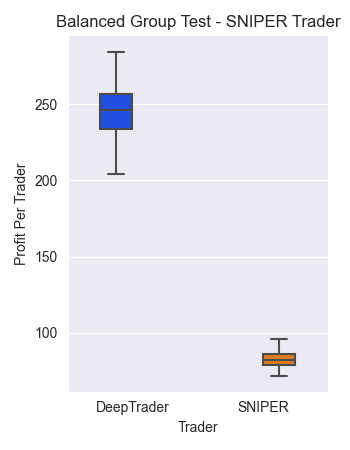
\includegraphics[width=.3\linewidth,height=120pt]{Balanced Group Test - SNIPER Trader.png}
%     \caption{Too much coffee.}
%   \end{tabular}
%   \begin{tabular}
%     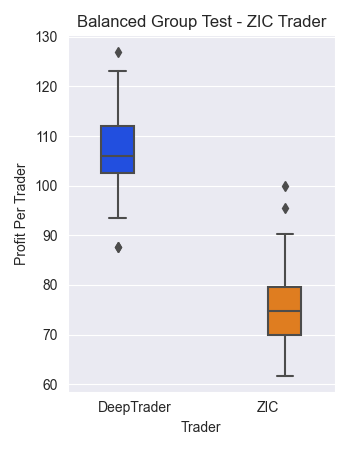
\includegraphics[width=.3\linewidth,height=120pt]{Balanced Group Test - ZIC Trader.png}
%     \caption{Too much coffee.}
%   \end{tabular}
%   \begin{tabular}
%     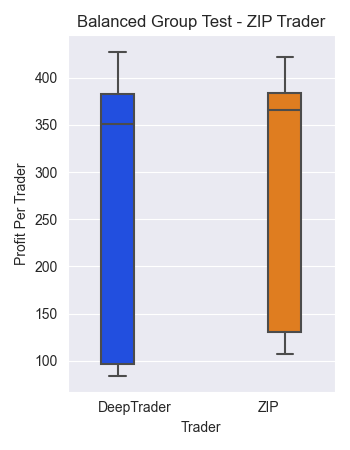
\includegraphics[width=.3\linewidth,height=120pt]{Balanced Group Test - ZIP Trader.png}
%     \caption{Too much coffee.}
%   \end{tabular}
%   \caption{Results for the Balanced Group Tests Comparing DeepTrader with Existing Trading Strategies.}
%   \label{fig:balanced_tests}
% \end{figure}

% {\bf A topic-specific chapter, of roughly $15$ pages} 
% \vspace{1cm} 

% \noindent
% This chapter is intended to describe what you did: the goal is to explain
% the main activity or activities, of any type, which constituted your work 
% during the project.  The content is highly topic-specific, but for many 
% projects it will make sense to split the chapter into two sections: one 
% will discuss the design of something (e.g., some hardware or software, or 
% an algorithm, or experiment), including any rationale or decisions made, 
% and the other will discuss how this design was realised via some form of 
% implementation.  

% This is, of course, far from ideal for {\em many} project topics.  Some
% situations which clearly require a different approach include:

% \begin{itemize}
% \item In a project where asymptotic analysis of some algorithm is the goal,
%       there is no real ``design and implementation'' in a traditional sense
%       even though the activity of analysis is clearly within the remit of
%       this chapter.
% \item In a project where analysis of some results is as major, or a more
%       major goal than the implementation that produced them, it might be
%       sensible to merge this chapter with the next one: the main activity 
%       is such that discussion of the results cannot be viewed separately.
% \end{itemize}

% \noindent
% Note that it is common to include evidence of ``best practice'' project 
% management (e.g., use of version control, choice of programming language 
% and so on).  Rather than simply a rote list, make sure any such content 
% is useful and/or informative in some way: for example, if there was a 
% decision to be made then explain the trade-offs and implications 
% involved.

% \section{Example Section}

% This is an example section; 
% the following content is auto-generated dummy text.
% \lipsum

% \subsection{Example Sub-section}

% \begin{figure}[t]
% \centering
% foo
% \caption{This is an example figure.}
% \label{fig}
% \end{figure}

% \begin{table}[t]
% \centering
% \begin{tabular}{|cc|c|}
% \hline
% foo      & bar      & baz      \\
% \hline
% $0     $ & $0     $ & $0     $ \\
% $1     $ & $1     $ & $1     $ \\
% $\vdots$ & $\vdots$ & $\vdots$ \\
% $9     $ & $9     $ & $9     $ \\
% \hline
% \end{tabular}
% \caption{This is an example table.}
% \label{tab}
% \end{table}

% \begin{algorithm}[t]
% \For{$i=0$ {\bf upto} $n$}{
%   $t_i \leftarrow 0$\;
% }
% \caption{This is an example algorithm.}
% \label{alg}
% \end{algorithm}

% \begin{lstlisting}[float={t},caption={This is an example listing.},label={lst},language=C]
% for( i = 0; i < n; i++ ) {
%   t[ i ] = 0;
% }
% \end{lstlisting}

% This is an example sub-section;
% the following content is auto-generated dummy text.
% Notice the examples in Figure~\ref{fig}, Table~\ref{tab}, Algorithm~\ref{alg}
% and Listing~\ref{lst}.
% \lipsum

% \subsubsection{Example Sub-sub-section}

% This is an example sub-sub-section;
% the following content is auto-generated dummy text.
% \lipsum

% \paragraph{Example paragraph.}

% This is an example paragraph; note the trailing full-stop in the title,
% which is intended to ensure it does not run into the text.

% % -----------------------------------------------------------------------------

\chapter{Critical Evaluation}
\label{chap:evaluation}

The intention of this chapter is to evaluate the performance of the DeepTrader agent against existing trading strategies. This will be achieved by providing a detailed analysis of the results from the experiments that were presented in Section \ref{sec:results}. For each test performed, this chapter will determine whether there is any statistically meaningful difference in the outcomes of the experiments for each trading strategy compared to DeepTrader under the various conditions. Where there is a significant difference, the evaluation will discuss which trading strategy is optimal.

\section{Confidence Interval}

The confidence interval $[c_{1}, c_{2}]$ for the mean $\bar{x}$ profit per trader produced by an experiment will be approximated. This will be done through the use of the central limit theorem see Equation \eqref{eq:confidence} where $s$ is the the standard deviation, $n$ is the number of samples and $Z_q$ is $q^{th}$-percentile of the standard normal distribution. The confidence intervals will be calculated using a significance level $\alpha= 0.1$. Therefore, $Z_{95} = 1.645$ and $n = 100$ in all cases. Analysis can be performed in this way as each sample drawn from an experiment is independent and there is a sufficient number of samples that have been drawn $n > 30$. 

\begin{equation}\label{eq:confidence} c_{1} = \bar{x} -  (Z_{1-\frac{\alpha}{2}} * \frac{s}{\sqrt{n}}),\; \, c_{2} = \bar{x} + (Z_{1-\frac{\alpha}{2}} * \frac{s}{\sqrt{n}})\end{equation}


\section{Comparisons with AA}
\subsection{Balanced Group Comparison}
Table \ref{table:bAA} displays the mean, standard deviation and 90\% confidence interval for the profit per trader of $100$ samples from the balanced group tests between AA and DeepTrader. DeepTrader's upper bound estimate of the mean profit per trader $c_2$ is less than AA's lower bound estimate of the mean profit per trader $c_1$. Therefore, at a 90\% confidence level there is enough statistical evidence to suggest that AA outperforms DeepTrader in a market where both AA and DeepTrader each account for 50\% of the market.

\begin{table}[H]
    \centering
    \begin{tabular}{c c c c c}
        \hline
        \textbf{Trader} & $\bar{x}$ & $s$ & $c_1$ & $c_2$ \\
        \hline
        DeepTrader & 249.1 & 17.86 & 246.2 & 252.0 \\ 
\rowcolor{lightgray} AA & 281.7& 15.74 & 279.1 & 284.3 \\ 
       
        \hline
    \end{tabular}

    \caption{Displays results from the Balanced Group Tests with DeepTrader and AA.}
    \label{table:bAA}
\end{table}

\subsection{One In Many Comparison}
Table \ref{table:oAA} displays the mean, standard deviation and 90\% confidence interval for the profit per trader of $100$ samples from the one in many tests between AA and DeepTrader. AA's upper bound estimate of the mean profit per trader $c_2$ is less than DeepTrader's lower bound estimate of the mean profit per trader $c_1$. Therefore, at a 90\% confidence level there is enough statistical evidence to suggest that DeepTrader outperforms AA when AA is the widely used strategy and DeepTrader is the minority. However, it is important to identify that DeepTrader has a large standard deviation for the samples in this test. Comparatively, AA has a very small standard deviation. The large standard deviation indicates that the profit per trader obtained from each experiment are spread far from the mean. Thus, DeepTrader outperforms AA in this setting but with a high variability.

\begin{table}[H]
    \centering
    \begin{tabular}{c c c c c}
        \hline
        \textbf{Trader} & $\bar{x}$ & $s$ & $c_1$ & $c_2$ \\
        \hline
        DeepTrader & 404.2 & 73.9 & 392.0 & 416.4 \\ 
\rowcolor{lightgray} AA & 301.2& 3.930 & 300.5 & 301.8 \\ 
       
        \hline
    \end{tabular}

    \caption{Displays results from the One In Many Tests with DeepTrader and AA.}
    \label{table:oAA}
\end{table}
\section{Comparisons with GDX}
\subsection{Balanced Group Comparison}
Table \ref{table:bGDX} displays the mean, standard deviation and 90\% confidence interval for the profit per trader of $100$ samples from the balanced group tests between GDX and DeepTrader. GDX's upper bound estimate of the mean profit per trader $c_2$ is less than DeepTrader's lower bound estimate of the mean profit per trader $c_1$. Therefore, at a 90\% confidence level the evidence demonstrates that DeepTrader is better than GDX in a market where both GDX and DeepTrader each account for 50\% of the market.

\begin{table}[H]
    \centering
    \begin{tabular}{c c c c c}
        \hline
        \textbf{Trader} & $\bar{x}$ & $s$ & $c_1$ & $c_2$ \\
        \hline
           DeepTrader & 284.8 & 30.31 & 279.8  & 289.7 \\ 
\rowcolor{lightgray} GDX &116.9 & 20.44 & 113.5 & 120.2 \\ 
       
        \hline
    \end{tabular}

    \caption{Displays results from the Balanced Group Tests with DeepTrader and GDX.}
    \label{table:bGDX}
\end{table}
\subsection{One In Many Comparison}
Table \ref{table:oGDX} displays the mean, standard deviation and 90\% confidence interval for the profit per trader of $100$ samples from the one in many tests between GDX and DeepTrader. GDX's upper bound estimate of the mean profit per trader $c_2$ is less than DeepTrader's lower bound estimate of the mean profit per trader $c_1$. Therefore, at a 90\% confidence level the evidence indicates that DeepTrader is better than GDX in a market where GDX is the vast majority of trading agents and DeepTrader is the minority.

\begin{table}[H]
    \centering
    \begin{tabular}{c c c c c}
        \hline
        \textbf{Trader} & $\bar{x}$ & $s$ & $c_1$ & $c_2$ \\
        \hline
        DeepTrader & 367.3 & 72.06 & 355.4 & 379.1 \\ 
\rowcolor{lightgray} GDX & 123.5 & 31.52 & 118.3 & 128.7 \\ 
       
        \hline
    \end{tabular}

    \caption{Displays results from the One In Many Tests with DeepTrader and GDX.}
    \label{table:oGDX}
\end{table}

\section{Comparisons with Giveaway}
\subsection{Balanced Group Comparison}
Table \ref{table:bGiveaway} displays the mean, standard deviation and 90\% confidence interval for the profit per trader of $100$ samples from the balanced group tests between Giveaway and DeepTrader. The mean profit per trader for DeepTrader lies inside of the 90\% confidence interval of Giveaway. Similarly, the mean profit per trader for Giveaway lies inside of the 90\% confidence interval of DeepTrader. Therefore, at a confidence level of 90\% there is no statistical evidence to suggest that there is a difference in performance between these two traders in a balanced group test.

\begin{table}[H]
    \centering
    \begin{tabular}{c c c c c}
        \hline
        \textbf{Trader} & $\bar{x}$ & $s$ & $c_1$ & $c_2$ \\
        \hline
           DeepTrader & 240.0 & 75.43 & 227.6 & 252.4\\ 
\rowcolor{lightgray} Giveaway & 234.1 & 56.50 & 224.8 & 243.4\\ 
       
        \hline
    \end{tabular}

    \caption{Displays results from the Balanced Group Tests with DeepTrader and Giveaway.}
    \label{table:bGiveaway}
\end{table}
\subsection{One In Many Comparison}
Table \ref{table:oGiveaway} displays the mean, standard deviation and 90\% confidence interval for the profit per trader of $100$ samples from the one in many tests between Giveaway and DeepTrader. Giveaway's upper bound estimate of the mean profit per trader $c_2$ is less than DeepTrader's lower bound estimate of the mean profit per trader $c_1$. Therefore, at a 90\% confidence level the statistical evidence shows that DeepTrader is better than Giveaway in a market where Giveaway is the vast majority of trading agents and DeepTrader is the minority.
\begin{table}[H]
    \centering
    \begin{tabular}{c c c c c}
        \hline
        \textbf{Trader} & $\bar{x}$ & $s$ & $c_1$ & $c_2$ \\
        \hline
        DeepTrader &400.9 & 68.19 & 389.7 & 412.2\\ 
\rowcolor{lightgray} Giveaway & 301.9 & 5.313 & 301.0 & 302.7 \\ 
       
        \hline
    \end{tabular}

    \caption{Displays results from the One In Many Tests with DeepTrader and Giveaway.}
    \label{table:oGiveaway}
\end{table}

\section{Comparisons with Shaver}
\subsection{Balanced Group Comparison}
Table \ref{table:bshav} displays the mean, standard deviation and 90\% confidence interval for the profit per trader of $100$ samples from the balanced group tests between Shaver and DeepTrader. Shaver's upper bound estimate of the mean profit per trader $c_2$ is less than DeepTrader's lower bound estimate of the mean profit per trader $c_1$. Therefore, at a 90\% confidence level the statistical evidence demonstrates that DeepTrader is better than Shaver in a market where both Shaver and DeepTrader each account for 50\% of the market.

\begin{table}[H]
    \centering
    \begin{tabular}{c c c c c}
        \hline
        \textbf{Trader} & $\bar{x}$ & $s$ & $c_1$ & $c_2$ \\
        \hline
           DeepTrader & 410.1 & 21.26 & 406.6 & 413.6\\ 
\rowcolor{lightgray} Shaver & 400.5 & 18.18 & 397.5 & 403.5\\ 
       
        \hline
    \end{tabular}

    \caption{Displays results from the Balanced Group Tests with DeepTrader and Shaver.}
    \label{table:bshav}
\end{table}
\subsection{One In Many Comparison}
Table \ref{table:oshav} displays the mean, standard deviation and 90\% confidence interval for the profit per trader of $100$ samples from the one in many tests between Shaver and DeepTrader. Shaver's upper bound estimate of the mean profit per trader $c_2$ is less than DeepTrader's lower bound estimate of the mean profit per trader $c_1$. Therefore, at a 90\% confidence level there is enough statistical evidence to suggest that DeepTrader outperforms Shaver when Shaver is the widely used strategy and DeepTrader is the minority. However, it is important to identify that DeepTrader has a large standard deviation for the samples in this test. Comparatively, Shaver has a very small standard deviation. The large standard deviation indicates that the profit per trader obtained from each experiment are spread far from the mean. Thus, DeepTrader outperforms Shaver in this setting but with a high variability.

\begin{table}[H]
    \centering
    \begin{tabular}{c c c c c}
        \hline
        \textbf{Trader} & $\bar{x}$ & $s$ & $c_1$ & $c_2$ \\
        \hline
        DeepTrader& 449.1 & 66.65 & 438.1 & 460.1\\ 
\rowcolor{lightgray} Shaver & 270.5 & 10.29 & 268.8 & 272.2 \\ 
       
        \hline
    \end{tabular}

    \caption{Displays results from the One In Many Tests with DeepTrader and Shaver.}
    \label{table:oshav}
\end{table}

\section{Comparisons with Sniper}
\subsection{Balanced Group Comparison}
Table \ref{table:bsnip} displays the mean, standard deviation and 90\% confidence interval for the profit per trader of $100$ samples from the balanced group tests between Sniper and DeepTrader. Sniper's upper bound estimate of the mean profit per trader $c_2$ is less than DeepTrader's lower bound estimate of the mean profit per trader $c_1$. Therefore, at a 90\% confidence level the statistical evidence demonstrates that DeepTrader outperforms Sniper in a market where both Sniper and DeepTrader each account for 50\% of the market.

\begin{table}[H]
    \centering
    \begin{tabular}{c c c c c}
        \hline
        \textbf{Trader} & $\bar{x}$ & $s$ & $c_1$ & $c_2$ \\
        \hline
           DeepTrader & 246.0 & 17.03 & 243.2 & 248.8\\ 
\rowcolor{lightgray} Sniper & 82.59 & 5.236 & 81.72 & 83.45\\ 
       
        \hline
    \end{tabular}

    \caption{Displays results from the Balanced Group Tests with DeepTrader and Sniper.}
    \label{table:bsnip}
\end{table}
\subsection{One In Many Comparison}
Table \ref{table:osnip} displays the mean, standard deviation and 90\% confidence interval for the profit per trader of $100$ samples from the one in many tests between Sniper and DeepTrader. Sniper's upper bound estimate of the mean profit per trader $c_2$ is less than DeepTrader's lower bound estimate of the mean profit per trader $c_1$. Therefore, at a 90\% confidence level there is enough statistical evidence to suggest that DeepTrader outperforms Sniper when Sniper is the widely used strategy and DeepTrader is the minority. However, it is important to identify that DeepTrader has a large standard deviation for the samples in this test. Comparatively, Sniper has a very small standard deviation. The large standard deviation indicates that the profit per trader obtained from each experiment are spread far from the mean. Thus, DeepTrader outperforms Sniper in this setting but with a high variability.

\begin{table}[H]
    \centering
    \begin{tabular}{c c c c c}
        \hline
        \textbf{Trader} & $\bar{x}$ & $s$ & $c_1$ & $c_2$ \\
        \hline
        DeepTrader & 89.71 & 32.21 & 84.41 & 95.01\\ 
\rowcolor{lightgray} Sniper & 74.28 & 6.854 & 73.16 & 75.41\\ 
       
        \hline
    \end{tabular}

    \caption{Displays results from the One In Many Tests with DeepTrader and Sniper.}
    \label{table:osnip}
\end{table}

\section{Comparisons with ZIC}
\subsection{Balanced Group Comparison}
Table \ref{table:bzic} displays the mean, standard deviation and 90\% confidence interval for the profit per trader of $100$ samples from the balanced group tests between ZIC and DeepTrader. ZIC's upper bound estimate of the mean profit per trader $c_2$ is less than DeepTrader's lower bound estimate of the mean profit per trader $c_1$. Therefore, at a 90\% confidence level the statistical evidence demonstrates that DeepTrader outperforms ZIC in a market where both ZIC and DeepTrader each account for 50\% of the market.

\begin{table}[H]
    \centering
    \begin{tabular}{c c c c c}
        \hline
        \textbf{Trader} & $\bar{x}$ & $s$ & $c_1$ & $c_2$ \\
        \hline
           DeepTrader & 106.7 & 7.459 & 105.5 & 107.9\\ 
\rowcolor{lightgray} ZIC & 75.37 & 7.458 & 74.14 & 76.60\\ 
       
        \hline
    \end{tabular}

    \caption{Displays results from the Balanced Group Tests with DeepTrader and ZIC.}
    \label{table:bzic}
\end{table}
\subsection{One In Many Comparison}
Table \ref{table:ozic} displays the mean, standard deviation and 90\% confidence interval for the profit per trader of $100$ samples from the one in many tests between ZIC and DeepTrader. ZIC's upper bound estimate of the mean profit per trader $c_2$ is less than DeepTrader's lower bound estimate of the mean profit per trader $c_1$. Therefore, at a 90\% confidence level there is enough statistical evidence to suggest that DeepTrader outperforms ZIC when ZIC is the widely used strategy and DeepTrader is the minority. However, it is important to highlight that DeepTrader has a large standard deviation for the samples in this test. Comparatively, ZIC has a very small standard deviation. The large standard deviation indicates that the profit per trader obtained from each experiment are spread far from the mean. Thus, DeepTrader outperforms ZIC in this setting but with a high variability.

\begin{table}[H]
    \centering
    \begin{tabular}{c c c c c}
        \hline
        \textbf{Trader} & $\bar{x}$ & $s$ & $c_1$ & $c_2$ \\
        \hline
        DeepTrader & 366.1 & 54.69 & 357.1 & 375.1\\ 
\rowcolor{lightgray} ZIC & 224.1 & 6.113 & 223.1 & 225.1 \\ 
       
        \hline
    \end{tabular}

    \caption{Displays results from the One In Many Tests with DeepTrader and ZIC.}
    \label{table:ozic}
\end{table}

\section{Comparisons with ZIP}
\subsection{Balanced Group Comparison}
Table \ref{table:bzip} displays the mean, standard deviation and 90\% confidence interval for the profit per trader of $100$ samples from the balanced group tests between ZIP and DeepTrader. The mean profit per trader for DeepTrader lies inside of the 90\% confidence interval of ZIP. Similarly, the mean profit per trader for ZIP lies inside of the 90\% confidence interval of DeepTrader. Therefore, at a confidence level of 90\% there is no statistical evidence to suggest that there is a difference in performance between these two traders in a balanced group test.

\begin{table}[H]
    \centering
    \begin{tabular}{c c c c c}
        \hline
        \textbf{Trader} & $\bar{x}$ & $s$ & $c_1$ & $c_2$ \\
        \hline
           DeepTrader & 245.0 & 144.7 & 221.2 & 268.8\\ 
\rowcolor{lightgray} ZIP & 263.1 & 128.9 & 241.9 & 284.3\\ 
       
        \hline
    \end{tabular}

    \caption{Displays results from the Balanced Group Tests with DeepTrader and ZIP.}
    \label{table:bzip}
\end{table}
\subsection{One In Many Comparison}
Table \ref{table:ozip} displays the mean, standard deviation and 90\% confidence interval for the profit per trader of $100$ samples from the one in many tests between ZIP and DeepTrader. ZIP's upper bound estimate of the mean profit per trader $c_2$ is less than DeepTrader's lower bound estimate of the mean profit per trader $c_1$. Therefore, at a 90\% confidence level there is enough statistical evidence to suggest that DeepTrader outperforms ZIP when ZIP is the widely used strategy and DeepTrader is the minority. However, it is important to identify that DeepTrader has a large standard deviation for the samples in this test. Comparatively, ZIP has a very small standard deviation. The large standard deviation indicates that the profit per trader obtained from each experiment are spread far from the mean. Thus, DeepTrader outperforms ZIP in this setting but with a high variability.

\begin{table}[H]
    \centering
    \begin{tabular}{c c c c c}
        \hline
        \textbf{Trader} & $\bar{x}$ & $s$ & $c_1$ & $c_2$ \\
        \hline
        DeepTrader & 318.5 & 63.40 & 308.1 & 328.9\\ 
\rowcolor{lightgray} ZIP & 277.4 & 12.10 & 275.4 & 279.4\\ 
       
        \hline
    \end{tabular}

    \caption{Displays results from the One In Many Tests with DeepTrader and ZIP.}
    \label{table:ozip}
    
    

\end{table}

\section{Summary of Results}
Table \ref{table:summary} and \ref{table:summary2} summarises the results by test approach for each trader strategy when compared against DeepTrader. As the table shows, DeepTrader was only outperformed by the AA trading strategy in the balanced group tests. More impressively, in the one in many tests, DeepTrader is shown to have outperformed all traders within the BSE.

It should be noted however, that particularly in the one in many tests the variability is high, suggesting that the DeepTrader outperforms another strategy but typically with a large difference in the amount it outperforms another strategy by.

\begin{table}[H]
    \centering
    \begin{tabular}{c ||c |c || }
      
        
        &\multicolumn{2}{c||}{Balanced Group}\\
        \hline
        & result & comment\\
        \hline
          AA & \cellcolor{red}$\downarrow$ & only test where DeepTrader was outperformed     \\
          GDX & \cellcolor{green}$\uparrow$ & DeepTrader significantly outperformed  \\
          Giveaway & \cellcolor{lightgray}- & no statistical difference in performance\\
          Shaver & \cellcolor{green}$\uparrow$ & DeepTrader outperformed  \\
          Sniper& \cellcolor{green}$\uparrow$ & DeepTrader significantly outperformed   \\
          ZIC& \cellcolor{green}$\uparrow$ & DeepTrader significantly outperformed \\
          ZIP & \cellcolor{lightgray}- & no statistical difference in performance \\
      
    \end{tabular}
    


    \caption{Summary of results for the Balanced Group tests.}
    \label{table:summary}
\end{table}

\begin{table}[H]
    \centering
    \begin{tabular}{c ||c |c || }
      
        
        &\multicolumn{2}{c||}{One In Many}\\
        \hline
        & result & comment\\
        \hline
          AA & \cellcolor{green}$\uparrow$ & DeepTrader outperformed but with a high variability \\
          GDX & \cellcolor{green}$\uparrow$ & DeepTrader significantly outperformed \\
          Giveaway & \cellcolor{green}$\uparrow$ & DeepTrader outperformed\\
          Shaver & \cellcolor{green}$\uparrow$ & DeepTrader outperformed but with a high variability  \\
          Sniper& \cellcolor{green}$\uparrow$ & DeepTrader outperformed but with a high variability  \\
          ZIC& \cellcolor{green}$\uparrow$ & DeepTrader outperformed but with a high variability \\
          ZIP & \cellcolor{green}$\uparrow$ & DeepTrader outperformed but with a high variability\\
      
    \end{tabular}
    


    \caption{Summary of results for the One In Many tests.}
    \label{table:summary2}
\end{table}
\section{Real World Application}

\subsection{Results}

It should be noted that the tests carried out in Section \ref{sec:results} do not completely imitate  real financial exchanges. Firstly, financial exchanges in the real world consist of a large number of different traders all acting within their own self interest. The trading strategies they use are often kept secret to ensure that they maximise any potential profit they earn and for these reasons, the assumption that an entire real world market can be modelled on only two types of trading strategy is implausible. Secondly, the buyer/seller distributions used for each trading strategy may be deemed to be unrealistic. In light of these points, the results obtained from the tests are promising but should be considered as preliminary. Therefore, whilst it can be concluded that these results present a direct comparison of the performance of DeepTrader against existing trading strategies within the public domain, they do not provide any indication of how DeepTrader will perform in the real world. 

\subsection{Availability of Limit Prices}

Section \ref{sec:features} outlined all the features that were extracted from BSE and used to train DeepTrader's LSTM network. All of this data is publicly available on a LOB based financial exchange, except for a trader's limit price. Naturally, a trader's limit price is always kept secret to maintain a competitive advantage over the other traders to maximise their profits and ensure that their position is not compromised by other traders. Hence, the capturing of limit price information when collecting and compiling the training data for this project can be considered impractical. 

Nevertheless, DeepTrader may still be implemented in a real world setting. A real world implementation of the DeepTrader strategy would require a history of (preferably profitable) trades where each of the 14 features listed in Section \ref{sec:features} are all captured. This could be done by the organisation or individual trader automating the collection of this information as they trade. After a sufficient amount of data (typically millions of data points) has been collected, the DeepTrader strategy can then be used to trade a real security. Whilst trading, the DeepTrader strategy like any other trading strategy is completely oblivious to another trader's limit price.


% {\bf A topic-specific chapter, of roughly $15$ pages} 
% \vspace{1cm} 

% \noindent
% This chapter is intended to evaluate what you did.  The content is highly 
% topic-specific, but for many projects will have flavours of the following:

% \begin{enumerate}
% \item functional  testing, including analysis and explanation of failure 
%       cases,
% \item behavioural testing, often including analysis of any results that 
%       draw some form of conclusion wrt. the aims and objectives,
%       and
% \item evaluation of options and decisions within the project, and/or a
%       comparison with alternatives.
% \end{enumerate}

% \noindent
% This chapter often acts to differentiate project quality: even if the work
% completed is of a high technical quality, critical yet objective evaluation 
% and comparison of the outcomes is crucial.  In essence, the reader wants to
% learn something, so the worst examples amount to simple statements of fact 
% (e.g., ``graph X shows the result is Y''); the best examples are analytical 
% and exploratory (e.g., ``graph X shows the result is Y, which means Z; this 
% contradicts [1], which may be because I use a different assumption'').  As 
% such, both positive {\em and} negative outcomes are valid {\em if} presented 
% in a suitable manner.

% -----------------------------------------------------------------------------

\chapter{Conclusion}
\label{chap:conclusion}

% {\bf A compulsory chapter,     of roughly $5$ pages} 
% \vspace{1cm} 

% \noindent
% The concluding chapter of a dissertation is often underutilised because it 
% is too often left too close to the deadline: it is important to allocation
% enough attention.  Ideally, the chapter will consist of three parts:

% \begin{enumerate}
% \item (Re)summarise the main contributions and achievements, in essence
%       summing up the content.
% \item Clearly state the current project status (e.g., ``X is working, Y 
%       is not'') and evaluate what has been achieved with respect to the 
%       initial aims and objectives (e.g., ``I completed aim X outlined 
%       previously, the evidence for this is within Chapter Y'').  There 
%       is no problem including aims which were not completed, but it is 
%       important to evaluate and/or justify why this is the case.
% \item Outline any open problems or future plans.  Rather than treat this
%       only as an exercise in what you {\em could} have done given more 
%       time, try to focus on any unexplored options or interesting outcomes
%       (e.g., ``my experiment for X gave counter-intuitive results, this 
%       could be because Y and would form an interesting area for further 
%       study'' or ``users found feature Z of my software difficult to use,
%       which is obvious in hindsight but not during at design stage; to 
%       resolve this, I could clearly apply the technique of Smith [7]'').
% \end{enumerate}
%
% \item Research and survey literature on existing automated trading agents.
% \item Build on work completed as part of the Applied Deep Learning Unit at Bristol, to further research into the use of RNNs.
% \item Implement a data pipeline for the collection and pre-processing of training data from BSE modelling a range of trading conditions.
% \item Create a profit making RNN which performs well under differing trading conditions. This will include defining its architecture and methodology, and how it should be initialised.
% \item Compare the performance of the new strategy with existing automated trading agents under the various trading conditions.

% =============================================================================

\section{Outcomes}
\label{sec:outcomes}
The main achievement of this project has been to devise a deep learning trading strategy that can trade competitively on a LOB based financial exchange against other existing well known trading strategies within the BSE. 

With respect to the aims and high level objectives that were introduced in Section \ref{sec:projectapproach}, the potential successes and shortcomings will be evaluated in turn below. To recap, those objectives  were:
\\
\begin{enumerate}

\item Research and survey literature on existing automated trading agents.
\item Build on work completed as part of the Applied Deep Learning Unit at Bristol, for further research into the use of RNNs.
\item Implement a data pipeline for the collection and pre-processing of training data from BSE modelling a range of trading conditions.
\item Create a profit making RNN which performs well under differing trading conditions. This will include defining its architecture and methodology, and how it should be initialised.
\item Compare the performance of the new strategy with existing automated trading agents under the various trading conditions.\\
\end{enumerate}

In regards to the first objective, detailed research and survey of the literature on existing automated trading agents was conducted and evidenced in Chapter \ref{chap:context} where an overview into the origins of experimental economics and publicly available automated trading agents was presented. 

Chapter \ref{chap:technical} went on to provide a detailed summary on the inner workings of all trading strategies that exist within BSE. It gave a more detailed treatment and investigation into the use of DLNNs in Section \ref{sec:deep} as well as a thorough description of how DLNNs work and how they could be applied for the purposes of this project.

Chapter \ref{chap:execution} began by outlining the approach taken to collect data and process it in a meaningful way for a DLNN in the BSE so that it could be used to model a range of trading conditions. It also described the network architecture of the DLNN, defined its input and described how this input will be used to trade. The tests conducted using the DeepTrader DLNN were described in Section \ref{sec:results}. This included specifying the types of tests that would be used to compare DeepTrader against the other trading strategies within BSE. 

Finally, the results from these tests were analysed in Chapter \ref{chap:evaluation}. The analysis demonstrated that DeepTrader was a competitive and profitable strategy against most traders in the BSE under most conditions. However, it also revealed that further work is necessary to understand why there was such high variability in profit taking under certain conditions and why there was no appreciable difference for some of the simpler training strategies (e.g. Giveaway).

Recalling the research hypothesis stated in the Executive Summary:\\
\begin{quote}
Does the use of DLNNs - specifically recurrent neural networks (RNNs) - and the additional parameters given by a LOB such as the quantities supplied or demanded at each price, and extended time series information on past bids and offers, let us train and create a trading agent that is comparably better than existing trading agents in the public literature?
\end{quote}

and in light of the accomplished objectives, DeepTrader has shown to be comparably better than most of the existing trading strategies under a prescribed set of testing conditions. However, the results presented in this paper do not provide a definitive answer to this question. In order to state this with a high level of confidence,  further work is necessary. This will include subjecting DeepTrader to an exhaustive set of comparison tests across a sufficiently wide range of market scenarios and providing a detailed analysis and critique of those findings.  \cite{snashall}.

\section{Future Work}

\subsection{Further Testing}

As highlighted in the previous section, a larger, comprehensive number of tests under a variety of different market conditions are need to properly answer the research hypothesis. Market conditions, where the types as well as proportions of different trading strategy, will need to be varied exhaustively to determine how often DeepTrader outperforms existing strategies. Fortunately, with the emergence of cloud computing such as Amazon's AWS, the resources and infrastructure required to conduct a large number of different market sessions are readily available, but extensive work will need to be carried out to configure the environment and data to model the conditions. Given the limited time available, it has been beyond the scope of this project to conduct such large conduct experiments.

\subsection{Training Data}

A well known phrase used within the field of machine learning  is ``garbage in, garbage out''. Essentially, this means that the performance of learning algorithms are heavily dependent on their input data. Put differently, the results gained from the algorithm are only as  good as the accuracy and volume of data supplied to it. To this end, an attempt has been made in this project, to provide information from a large number of trades collected from thousands of market sessions consisting of all trading strategies that were available within BSE.

Nevertheless, this may not be the most effective approach for creating a training dataset for DeepTrader. For example, this project used trading strategies that were known to be underperform such as ZIC. In practice, this may skew the data towards realistic scenarios and as as a consequence DeepTrader may only be performing well under this conditions. Therefore, further investigation and analysis needs to be completed as to what strategy or combination of strategies should be used for training DeepTrader.

Moreover, the BSE simulation may have particular biases compared to real world exchanges which inadvertently provide a favourable outcome for DeepTrader's performance. Hence it would be ideal to use training data from other stock exchanges simulations and even the real world.

\subsection{Feature Perturbation and Sensitivity Analysis}

Section \ref{sec:features} outlines the 13 different features that were used to train the network. One other area of investigation could be to perform a ``sensitivity analysis'' on these different features. This would involve varying each feature with respect to each other and then analysing the performance of DeepTrader. This for example, could be done in several ways when training the network, such as clamping one of the inputs to its normalised limits (0 or 1) or masking an input with random noise and then re-testing it against other traders. If there is no appreciable change in DeepTrader's performance then that would indicate that a specific feature is redundant.


\section{Final Words}
It is hoped that this project has demonstrated a novel and effective approach of using deep learning to create a profitable trading strategy. The intention is that the ideas from this project can be the catalyst for new research into using deep learning to trade on financial markets which could eventually become the most effective method of addressing the sales trader problem.
% =============================================================================
% Finally, after the main matter, the back matter is specified.  This is
% typically populated with just the bibliography.  LaTeX deals with these
% in one of two ways, namely
%
% - inline, which roughly means the author specifies entries using the 
%   \bibitem macro and typesets them manually, or
% - using BiBTeX, which means entries are contained in a separate file
%   (which is essentially a databased) then inported; this is the 
%   approach used below, with the databased being dissertation.bib.
%
% Either way, the each entry has a key (or identifier) which can be used
% in the main matter to cite it, e.g., \cite{X}, \cite[Chapter 2}{Y}.

\backmatter

\bibliography{dissertation}

\appendix

\chapter{Appendix}
\label{appx:example}
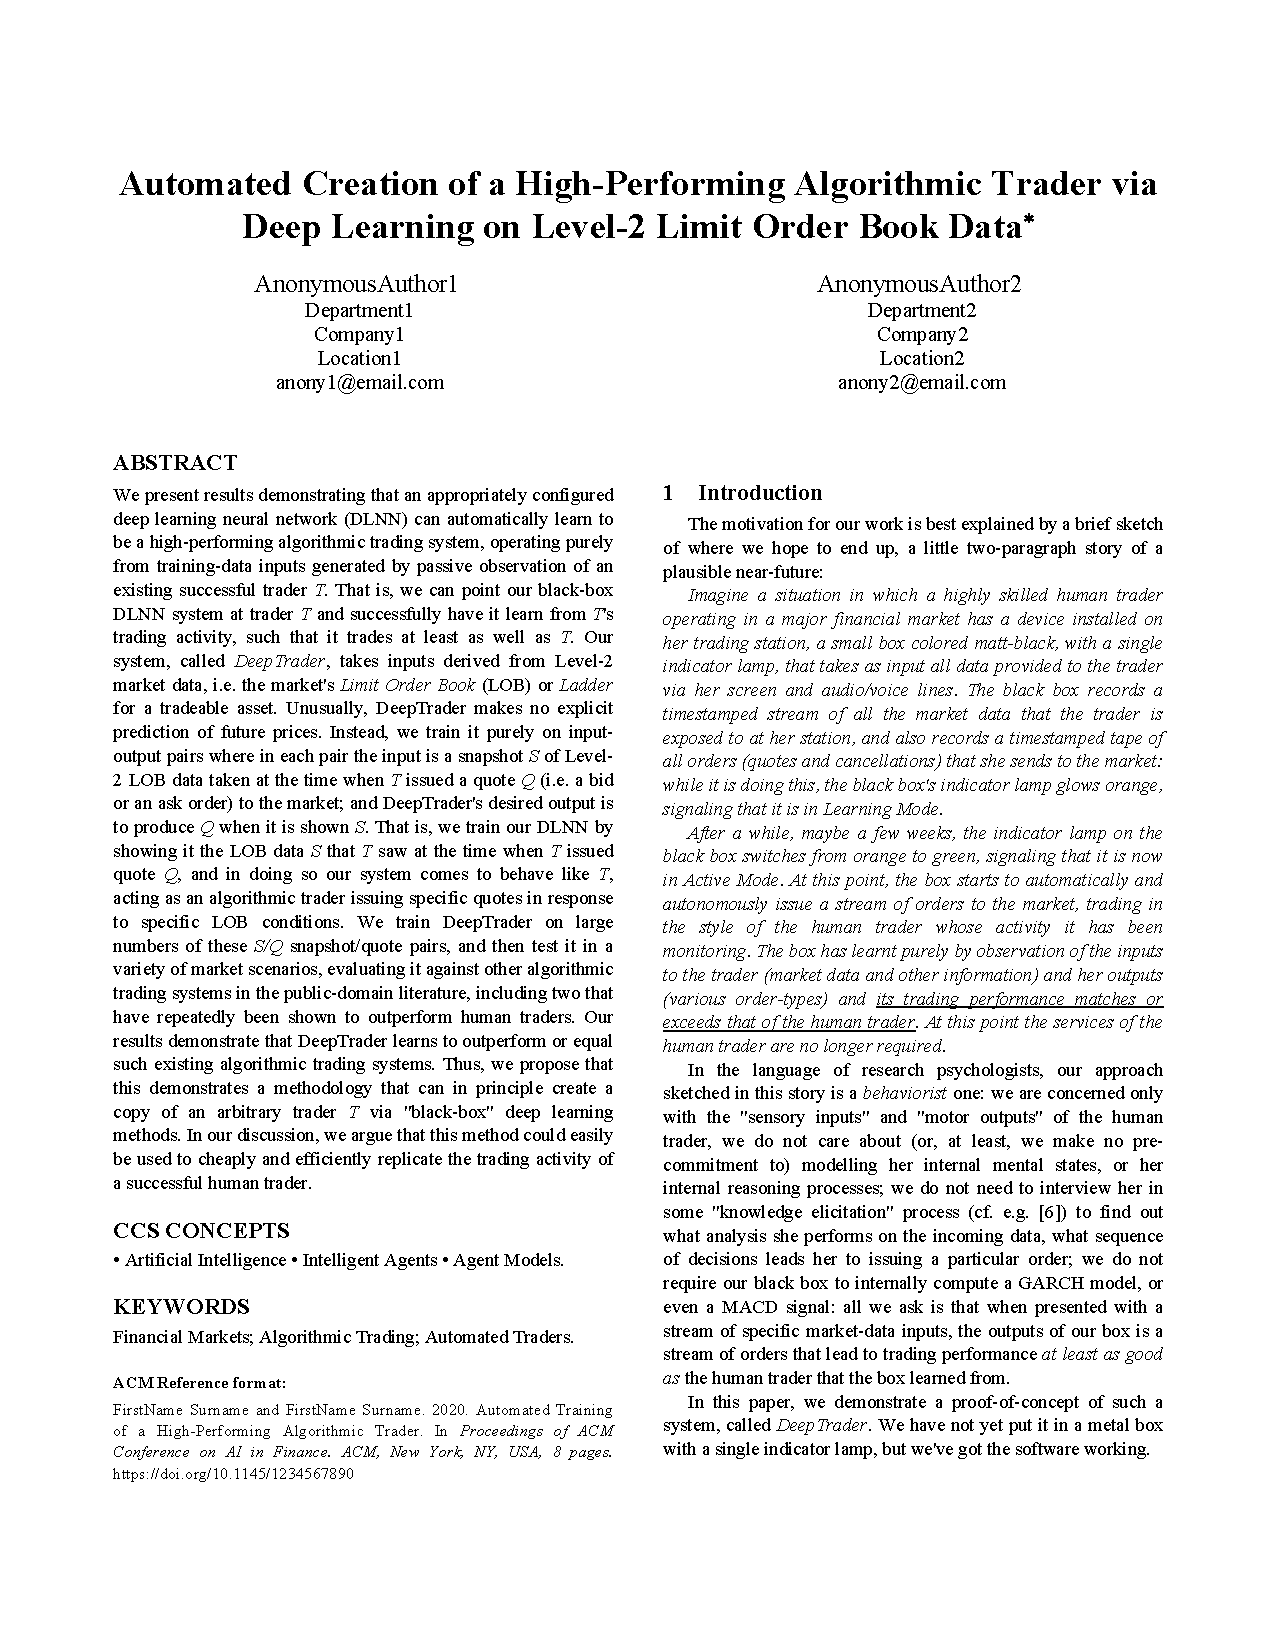
\includepdf[pages=-]{WrayCliff2020.pdf}


% -----------------------------------------------------------------------------

% The dissertation concludes with a set of (optional) appendicies; these are 
% the same as chapters in a sense, but once signaled as being appendicies via
% the associated macro, LaTeX manages them appropriatly.





% Content which is not central to, but may enhance the dissertation can be 
% included in one or more appendices; examples include, but are not limited
% to

% \begin{itemize}
% \item lengthy mathematical proofs, numerical or graphical results which 
%       are summarised in the main body,
% \item sample or example calculations, 
%       and
% \item results of user studies or questionnaires.
% \end{itemize}

% \noindent
% Note that in line with most research conferences, the marking panel is not
% obliged to read such appendices.

% =============================================================================

\end{document}
